\documentclass[11pt,a4paper]{article}

\usepackage{fullpage}
\usepackage{hyperref}
\usepackage{graphicx}
\usepackage{amsmath}
\usepackage{subfig}
\usepackage{todonotes}
\usepackage{amsthm}										            			                            %For not cursive theorems
\usepackage{framed}										            	                        		    %for frames around theorems
\usepackage{thmtools}											                                    		%for easy custom theorems
\usepackage{float}
\usepackage{amsfonts}
\usepackage[super]{nth}


\usepackage{fancyhdr}
\pagestyle{fancy}
\fancyhf{}

\renewcommand{\headrulewidth}{0pt}
\renewcommand{\footrulewidth}{0pt}

\fancypagestyle{firstpagefooter} {
	\lfoot{\tiny{Version: }}
	\cfoot{}
	\rfoot{\thepage}
}

\newcommand{\co}[1]{\texttt{#1}}
\newcommand{\ku}[1]{\textit{#1}}

%   \begin{mytitle}[Title] This is the text. \end{mytitle}
%	1 Title: This is the text.
\makeatletter
\declaretheoremstyle[
	spaceabove=6pt, spacebelow=6pt,
	headfont=\normalfont\bfseries,
	notefont=\color{black}\bfseries, 
	notebraces={}{},
	bodyfont=\normalfont,
	postheadspace=0.5 em,
	headpunct={:},
	spacebelow=\parsep,
    	spaceabove=\parsep,
	postheadhook={%
		},
	numberwithin=subsubsection,
]{mytitlesubsub}
\declaretheorem[name={}, style=mytitlesubsub]{mytitlesubsub}
\makeatother

%   \begin{mytitle}[Title] This is the text. \end{mytitle}
%	1 Title: This is the text.
\makeatletter
\declaretheoremstyle[
	spaceabove=6pt, spacebelow=6pt,
	headfont=\normalfont\bfseries,
	notefont=\color{black}\bfseries, 
	notebraces={}{},
	bodyfont=\normalfont,
	postheadspace=0.5 em,
	headpunct={:},
	spacebelow=\parsep,
    	spaceabove=\parsep,
	postheadhook={%
		},
	numberwithin=subsection,
]{mytitlesub}
\declaretheorem[name={}, style=mytitlesub]{mytitlesub}
\makeatother

%   \begin{mytitle}[Title] This is the text. \end{mytitle}
%	1 Title: This is the text.
\makeatletter
\declaretheoremstyle[
	spaceabove=6pt, spacebelow=6pt,
	headfont=\normalfont\bfseries,
	notefont=\color{black}\bfseries, 
	notebraces={}{},
	bodyfont=\normalfont,
	postheadspace=0.5 em,
	headpunct={:},
	spacebelow=\parsep,
    	spaceabove=\parsep,
	postheadhook={%
		},
	numberwithin=section,
]{mytitle}
\declaretheorem[name={}, style=mytitle]{mytitle}
\makeatother

\lfoot{Name: Ulla Aeschbacher Legi: 13-916-028}
\rfoot{\thepage}

\begin{document}

\title{Advanced Systems Lab Report\\ \normalsize{Autumn Semester 2018}}
\author{Name: Ulla Aeschbacher\\Legi: 13-916-028}
\date{
	\vspace{4cm}
	\textbf{Grading} \\
	\vspace{0.5cm}
	\begin{tabular}{|c|c|}
		\hline  \textbf{Section} & \textbf{Points} \\
		\hline  1                &                 \\ 
		\hline  2                &                 \\ 
		\hline  3                &                 \\ 
		\hline  4                &                 \\ 
		\hline  5                &                 \\ 
		\hline  6                &                 \\ 
		\hline  7                &                 \\ 
		\hline \hline Total      &                 \\
		\hline 
	\end{tabular} 
}
\maketitle
\thispagestyle{firstpagefooter}

\newpage

\section{System Overview (75 pts)}
Our middleware consists of four main parts: \co{MyMiddleware}, \co{NetThread}, \co{WorkerThread} and \co{ShutDownHook}. We will describe them all in detail below. In Figure \ref{Figure:threads} one can see all threads and important queues in our system and how they work together with the clients and servers. In Figure \ref{Figure:getset} the handling of GET and SET requests is shown. We will leave away the instrumentation when describing the main parts and will describe everything having to do with logging in its own section. 

\begin{figure}[!htb]
\centering
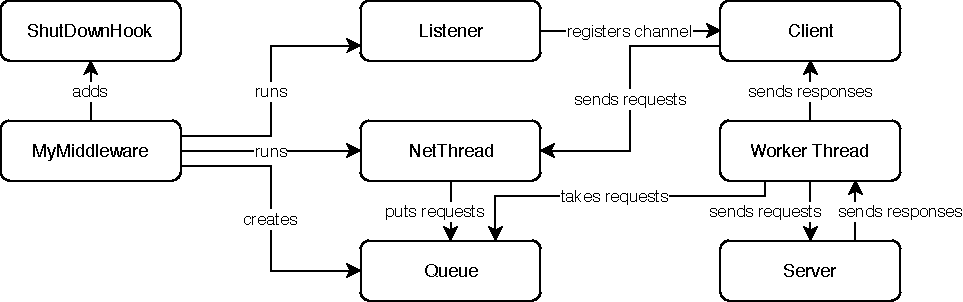
\includegraphics[scale=1]{graphics/threads.pdf}
\caption{\textit{Connection of all threads and queues.} An arrow from part A to part B means that A initializes this action.}
\label{Figure:threads}
\end{figure}

\begin{figure}[!htb]
\centering
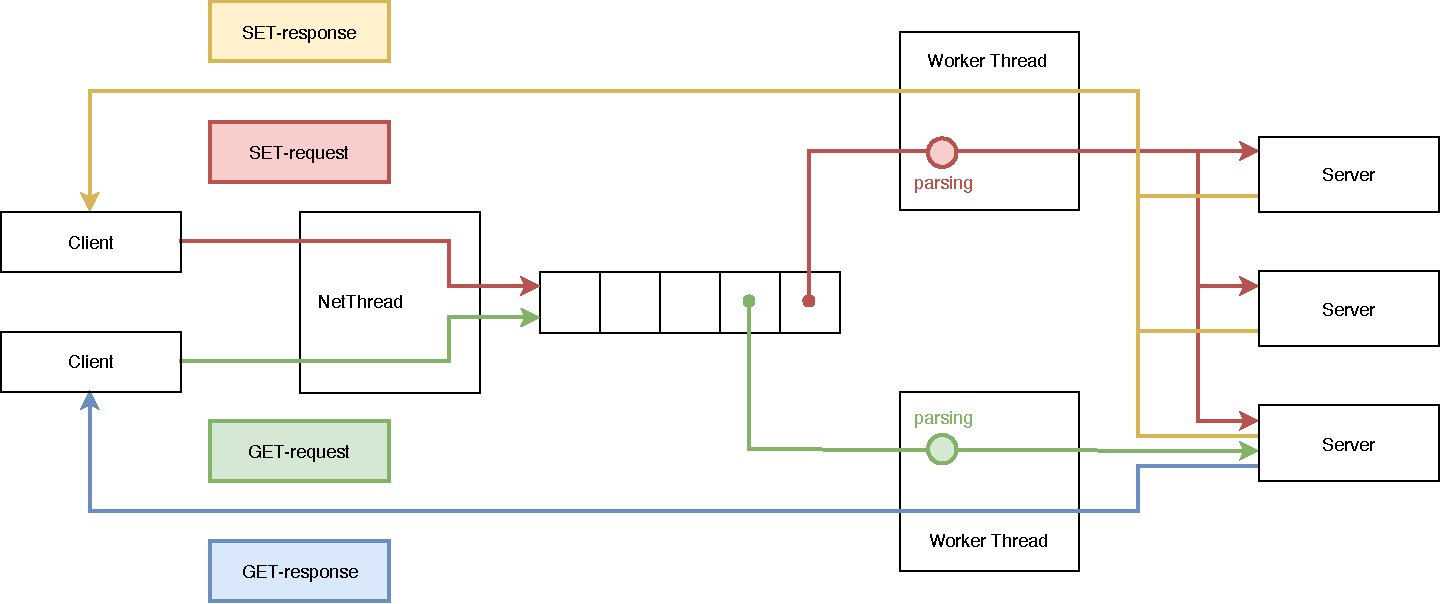
\includegraphics[width=\textwidth]{graphics/getset.pdf}
\caption{\textit{Handling of different requests.} Illustration on how two requests would go through the middleware.}
\label{Figure:getset}
\end{figure}

\subsection{MyMiddleware}
This thread gets called from \co{RunMW} and handles setup and breakdown of the middleware. In the constructor, we just add the \co{ShutDownHook}. Once run from \co{RunMW}, \co{MyMiddleware} opens a \co{Selector} and starts a new thread \co{Listener} which opens a nonblocking \co{ServerSocketChannel} on the address of the middleware. It creates \co{SocketChannel}s for connection requests. It also registers the new channels with the \co{Selector}, creating a \co{SelectionKey}. \co{MyMiddleware} then creates a \co{ThreadPoolExecutor} with a \co{LinkedBlockingQueue} for the \co{RequestHandler}s and a \co{WorkerThreadFactory} which creates the \co{WorkerThread}s that will handle the requests. The factory is given the server addresses such that \co{WorkerThread}s can use them in their initialization. Lastly, the middleware starts the \co{NetThread}.

\subsection{NetThread}
When the \co{NetThread} is run, it starts going through the channels from the \co{Selector} that are ready to be read from. For each readable \co{SelectionKey}, the \co{NetThread} creates a runnable \co{RequestHandler} and adds it to the \co{ThreadPoolExecutor}, which in turn adds the \co{RequestHandler} to his queue to be executed sometime in the future. The \co{ThreadPoolExecutor} then distributes the requests to the \co{WorkerThread}. To make sure that a key is not processed multiple times, we use a \co{HashSet} that contains all keys that are currently in the \co{ThreadPoolExecutor}. We remove a key from this set once we have sent the response to the request or the channel got closed. This is communicated by setting the attachment of the \co{SelectionKey} to different values.

\subsection{WorkerThread}
When a \co{WorkerThread} is created, it sets up \co{Socket}s and \co{BufferedReader}s for all the server addresses that were specified when the middleware was started. It saves them in two lists that remain for the whole lifetime of the middleware. We only create \co{WorkerThread}s at the beginning, up to the number specified when starting the middleware and then never kill them until the middleware is shut down. The assignment of \co{WorkerThread}s to requests in the queue is handled by the \co{ThreadPoolExecutor}. As soon as a \co{WorkerThread} gets assigned to a request, it runs the \co{RequestHandler} that is attached to that request. 

\subsubsection{RequestHandler}
The \co{RequestHandler} first creates a new \co{ReadRequestIntoBufferHandler} (see section \ref{readrequestLabel}) on the key, and gets back a \co{ByteBuffer} that has the complete request in it. If the buffer is empty, it changes the attachment of the \co{SelectionKey} to mark it as being done with processing, then the \co{Runnable} returns. Otherwise - after trimming the request of empty buffer space - it calls method \co{sendToServers} of the \co{WorkerThread} and receives back a \co{String} which is the response from the server. It puts this response into a \co{ByteBuffer}, flips the buffer and then writes the buffer to the \co{SocketChannel} until we have sent everything to the client. Having finished that, it changes the attachment of the \co{SelectionKey} to mark it as being done with processing and then returns.

\subsubsection{Communication with Servers}
The communication with the servers is all done in the \co{WorkerThread} because it can set up persistent connections, which would not be possible in the per-request \co{RequestHandler}. First, it figures out if the request whether a SET or a GET request by looking at the first three characters of the request. If it is neither of them, we log an error and return an empty string. Depending on what type of request has to be sent, \co{sendToServers} does something different. For SET requests we send the request to all servers and collect the responses. We then aggregate the responses into one by returning the first error or, in the case of no errors, returning "STORED". We then give that response back to the \co{RequestHandler}. For GET requests, we first have to figure out if it is a MULTI-GET request or not and if we are in the sharded or non-sharded case. For single GET requests and non-sharded MULTI-GET requests, we use a hash on the first key of the request to determine which server we send it to. To prove that the servers get an equal share of requests, we logged the number of requests each server handles. We give the result of one experiment run from experiment 5.2 in Table \ref{Table:1_proof} to prove this empirically.

\begin{table}[H]
	\centering
		\begin{tabular}{|r|r|r|} 
			\hline 		& Number of requests	& Percentage of whole workload\\			
			\hline Server 1   & 78198      					& 33.33844934 \%              \\ 
			\hline Server 2  	& 78177  						& 33.32949633 \%                   \\ 
			\hline Server 3 	& 78183                      	& 33.33205433 \%\\ 
			\hline 
		\end{tabular}
		\caption{\textit{Distribution of requests to the servers.}}
		\label{Table:1_proof}
\end{table}

The response from that server is then given back to the \co{RequestHandler}. For sharded MULTI-GET	requests, we first compute a large and small load with the following formulas. We use $numKeys$ as the number of keys in the request and $numServers$ as the number of servers we have running.
	\begin{equation}
	\begin{split}
		largeLoad = & \left\lceil\frac{numKeys}{numServers}\right\rceil\\
		smallLoad = & \left\lfloor\frac{numKeys}{numServers}\right\rfloor\\
		numLarge = & \text{ number of servers taking } largeLoad \text{ requests: } numKeys\ \%\ numServers\\
		numSmall = & \text{ number of servers taking } smallLoad \text{ requests: } \\
		& \left\{\begin{tabular}{l l l}
			$numKeys > numServers$ & $\Rightarrow$ & $numServers - numLarge$\\
			$else$ & $\Rightarrow$ & 0
		\end{tabular}\right.
	\end{split}
	\end{equation}
We then create all the smaller single GET or MULTI-GET commands that are needed and send them to the appropriate servers. After receiving a response from all of them, we combine them all into a single response and return that back to the \co{RequestHandler}. When reading from the servers, we always assume that there are no true carriage returns (i.e. ASCII 0D) in the response. Otherwise we could never be sure to have read the whole response.
\subsubsection{ReadRequestIntoBufferHandler} \label{readrequestLabel}
First of all, the \co{ReadRequestIntoBufferHandler} reads from the given channel into a \co{ByteBuffer}. If the number of bytes that was read is $-1$, we know that the channel has closed. We mark the \co{SelectionKey} associated to the channel as finished and return an empty buffer. Otherwise, we look at the first character of the buffer and based on that handle a SET or GET request. If it is neither of them, we log an error and return an empty buffer. If it is a valid request, we either call \co{handleGet} or \co{handleSet}.
\begin{itemize}
	\item \co{handleGet}: we look at the last character written to the buffer. If it is not a \co{$\backslash$n}, we know that we haven't read the full message yet. If the buffer is full we double the capacity of the buffer, then read from the channel  as soon as it is readable. Then we call \co{handleGet} again. We do this until the last character written to the buffer is a \co{$\backslash$n}.
	\item \co{handleSet}: we look at the last character written to the buffer. If it is not a \co{$\backslash$n} and the buffer is full, we double the capacity of the buffer, read from the channel and call \co{handleSet} again. Otherwise, we separate out the "bytes" element from the request and compare it to the length of the data block we have read thus far. If they do not match, we read on the channel until we have read data that is as long as the header of the request says. After that we are sure that we have a complete SET request in the buffer. 
\end{itemize}

\subsection{ShutDownHook}
The \co{ShutDownHook} shuts down the \co{ThreadPoolExecutor} and interrupts the \co{NetThread} and the \co{Listener}. Then it starts writing all the accumulated logs to files. After it has finished logging, it also shuts down the Logger.

\subsection{Instrumentation}
We have a Singleton class \co{Collector} that stores a \co{ThreadLocal<LinkedBlockingQueue\\<CollectorFile>>} for each thread. Each thread puts its logs into his queue in the form of \co{CollectorFile}s. Such an object stores the time it was created, the type of statistic it contains, optionally the operation type (i.e. GET, SET or MULTI-GET) and optionally a string containing the value. The \co{ShutDownHook} then goes through all the queues and separates them into \co{ArrayList}s per type of statistic. We then aggregate these values per a log window (standard five seconds). After that, \co{Log4j}s \co{LogManager.getFormatterLogger()} \footnote{https://logging.apache.org/log4j/2.x} is used to get a logger. We use a \co{Log4jMarker} per statistic type to write all the logs into files. The marker makes sure that each type of statistic is written to a separate file. We log eight different values.
\begin{itemize}
	\item Throughput: We measure the throughput by creating a new \co{CollectorFile} each time we have finished processing a request, i.e. sent back a response. When aggregating, we separate the values per operation type. We then count how many logs there are in the log window and divide them by the length of the log window. This gives us the throughput.
	\item Queue length: We measure the queue length everytime we put a new element into the queue. When aggregating, we take the average of all values that were logged in the log window. 
	\item Queue wait time: We measure the queue wait time as the difference between the time we create the \co{RequestHandler} for the request and the time the \co{RequestHandler} gets run on this request. To enable this, each \co{RequestHandler} gets the timestamp when it was created as an argument. When aggregating, we take the average of all values that were logged in the log window. 
	\item Server wait time: We measure the server wait time as the difference between the time we write the request to the output stream of the server and the time we read the first line from the server. If we sent the request to multiple servers, we take the longest wait time. We also note in the log how many keys were in the request, which is important for MULTI-GETs. When aggregating, we use this data for two things. First, to get latencies aggregated over the log window. For this we separate the values per operation type. We then divide the time by the number of requests and take the average of all those values that were logged in the log window. Second, to get data similar to the histogram data given by memtier.
	\item Server assigns: Whenever we have sent requests to servers, we log how many single requests we have sent to each one. When aggregating, we sum them up per log window. This is used to prove that we distribute the requests evenly.
	\item Number of requests: We measure the number of requests by creating a new \co{CollectorFile} just before we send the request to the server. When aggregating, we separate the values per operation type. We then count how many logs there are in the log window. 
	\item Cache misses: We measure the cache misses by comparing the number of requests we sent to a server with the number of non-empty responses we got and log the difference if it is greater than zero. When aggregating, we take the average of all values that were logged in the log window. 
	\item Errors: We log several errors. In the \co{Listener} we log a \co{ClosedByInterruptException} caused by interrupting the \co{Listener} in the \co{ShutDownHook}. We also log an \co{IOException} caused by various commands related to setting up the socket channels. In the \co{NetThread} we also log a \co{ClosedByInterruptException} and a \co{CancelledKeyException}, both caused by interrupting the \co{NetThread} in the \co{ShutDownHook}. In the \co{RequestHandler} there is again a \co{CancelledKeyException}, caused by he \co{ShutDownHook}. Lastly we also log the case where we get an unsupported message, which is just a message not starting with 'g' or 's'. Because we can assume that memtier only creates viable requests, this error should never be relevant.
\end{itemize}

\subsection{Experiments and Graph Generation}
We run our experiments on virtual machines with different amounts of cores. We have one core on each server VM, two cores on each client VM and four cores on each middleware VM. We know through \ku{iperf} that one core has a bandwidth of around 12.5 MB/s. We assume that a GET-request has around 300 Bytes and a response to it has around 4300 Bytes. We assume that a SET-request has around 4300 Bytes and a response to it has around 100 Bytes. We use these numbers when arguing about how many requests/responses a VM can send. 

From now on, an experiment run stands for a memtier command that is executed on each of the clients simultaneously. At the beginning of every experiment run, we run pings from each client to each of the servers, so that we can see if there are irregularities in the network. During the experiment run, dstat runs on each of the virtual machines used and collects statistics about the machine.

Each experiment run has a test-time of 70 seconds, of which we omit 5 seconds each as startup and cooldown-phase to get an actual plot time of one minute. 

For all experiments it holds:
\begin{equation}
	\begin{split}
	numClients 	= & numMemtier \cdot CPM \\
						= & numVMs \cdot numInstances \cdot numThreads \cdot numVirtualClients\\
	\end{split}
\end{equation}
When writing clients, we refer to this number.
We calculated the average and standard deviation over all files with the same \ku{numClients}. For throughput, we also multiply these values with \ku{numClients}, so that we get the total throughput and not the throughput per virtual client.  

The interactive law for experiment is computed as:
\begin{equation}
	throughput = \frac{numClients}{responseTime + thinkingTime }
\end{equation}
We always assume \ku{thinkingTime} to be zero.

\section{Baseline without Middleware (75 pts)}
In this section we did measurements on the throughput and latency of memtier requests without a middleware. The numbers come from the logs that memtier provides as well as from dstat.
\subsection{One Server}
The parameters are as in Table \ref{Table:2_1_table}. Throughput and response time are plotted in Figure \ref{Figure:2_1}. 

	\begin{table}[H]
	\centering
		\begin{tabular}{|l|c|} 
			\hline Number of servers                				& 1                        \\ 
			\hline Number of client machines        		& 3                        \\ 
			\hline Instances of memtier per machine 	& 1                        \\ 
			\hline Threads per memtier instance     		& 2                        \\
			\hline Virtual clients per thread       			& 1, 2, 4, 8, 16, 32, 64, 128                 \\ 
			\hline Workload                         					& Write-only and Read-only \\
			\hline Repetitions                      					& 3                 \\ 
			\hline 
		\end{tabular}
		\caption{\textit{Parameters for experiment 2.1}}
		\label{Table:2_1_table}
	\end{table}


\begin{figure}[t!]
	\subfloat[Throughput]{
		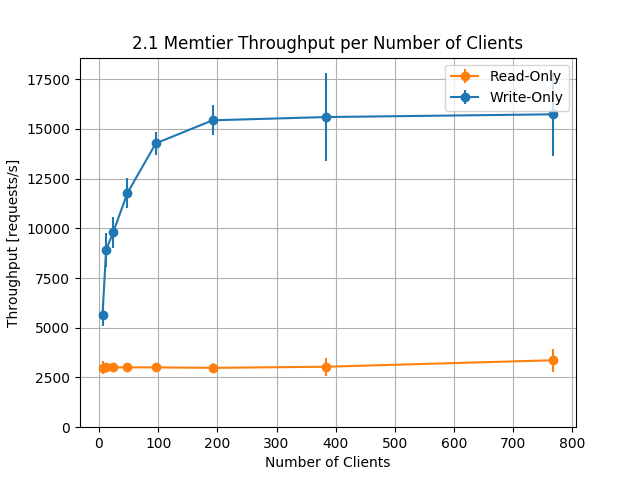
\includegraphics[width=0.5\linewidth]{figures/2_1_Memtier_Throughput_per_Number_of_Clients.png}
		\label{Figure:2_1:a}}\hfill
	\subfloat[Response time]{
		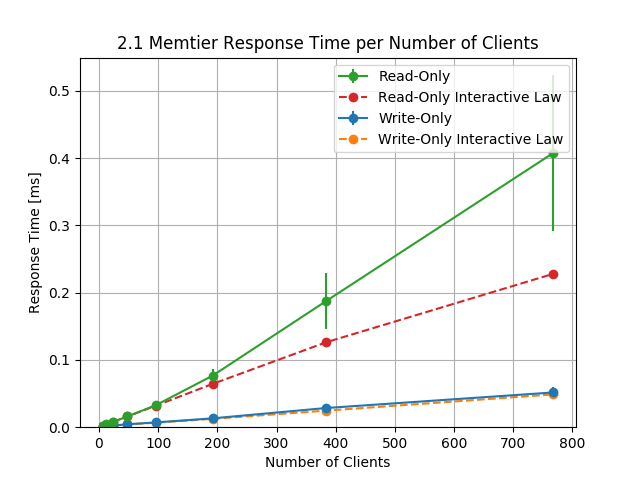
\includegraphics[width=0.5\linewidth]{figures/2_1_Memtier_Response_Time_per_Number_of_Clients.png}
		\label{Figure:2_1:b}}\\
	\subfloat[Network Read-Only]{
		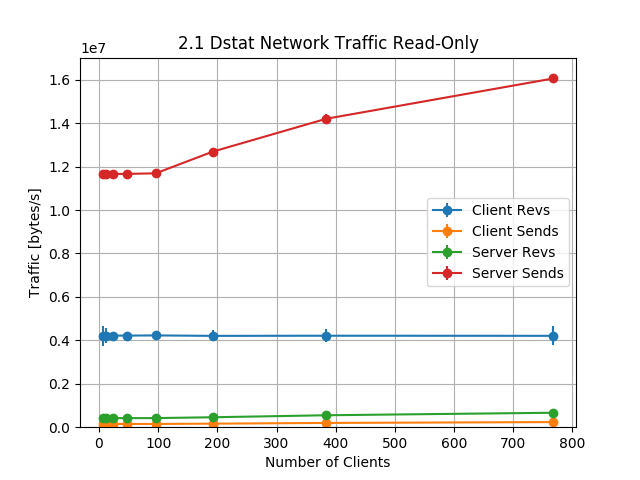
\includegraphics[width=0.5\linewidth]{figures/2_1_Dstat_Network_Traffic_Read-Only.png}
		\label{Figure:2_1_dstat:a}}\hfill
	\subfloat[CPU Write-Only]{
		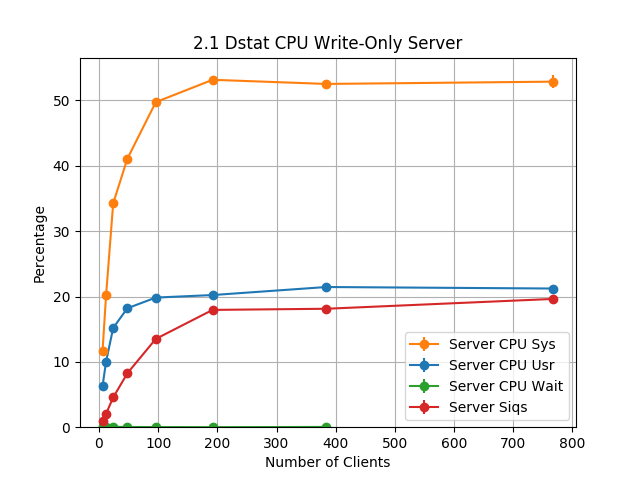
\includegraphics[width=0.5\linewidth]{figures/2_1_Dstat_CPU_Write-Only_Server.png}
		\label{Figure:2_1_dstat:b}}\\
	\caption{\textit{Plots for experiment 2.1.} Averaged throughput and latency values for both a read-only and a write-only load. Also average of the network inbound and outbound traffic for clients and servers for the read-only workload and average of the CPU usage for the server for the write-only workload.}
	\label{Figure:2_1} 	
\end{figure}

\subsubsection{Explanation}

\mytitlesubsub[Read-Only Workload]{In this graph, the throughput (see Figure \ref{Figure:2_1:a}) seems steady until 384 clients, then it increases just a bit for 768 clients. Even when looking at a more detailed graph, we can't see the inflection point. Thus the system is saturated right from the start. The interactive law (see Figure \ref{Figure:2_1:b}) holds quite well until we get to 192 clients, from then on our response times get bigger than what the law predicts. This can happen when we have some outliers with a very long response time. They do not show up in the throughput, becaus we have so many clinets sending at the same time, but they will increase our response time average. That is also why the error bars for those measurements are bigger. We would think that the bottleneck is in the server, because we only have one server versus three clients. When we look at the bandwidth of around 12.5 MB/s per core of a VM, we know that all three clients together with two cores each can thus send around 75 MB/s and the server with one core can send 12.5 MB/s. A read-only request sent from the client is very short but the response the server has to send back is very long. The clients together can thus send around 250'000 requests/second. We can also roughly calculate the number of responses the server can maximally send back as around 2900. Thus the bottleneck is clearly at the server. This matches what we measured, with an average throughput of 3000 requests/second. Because of this we would also expect the server outbound traffic to be highest. From the network traffic observed on the virtual machines (see Figure \ref{Figure:2_1_dstat:a}) we can see this hypothesis confirmed.}
\mytitlesubsub[Write-Only Workload]{The throughput (see Figure \ref{Figure:2_1:a}) climbs steeply until 96 clients, which suggests that the system is undersaturated until then. From then on the throughput stays the same which means that the system is saturated; we do not reach a point where the system is oversaturated. We can see the same behaviour in the response time graph (see Figure \ref{Figure:2_1:b}), where there is a small change in steepness at 96 clients. The interactive law holds extremely well, we can barely see a difference. For a write-only workload what the client sends is very long while the server has to send back either an error or success message, which is really short. Thus the server can handle sending back around 125'000 responses/second, but the clients can together only send around 17'400 requests/second.  Thus, we would think that the bottleneck is at the clients. But when looking at the measured data we see that our maximum throughput is only around 15'700 requests/second. Our bottleneck could be in the CPU and not in the bandwidth of a virtual machine. Looking at the CPU usage observed on the server VM (see Figure \ref{Figure:2_1_dstat:b}) we can see that the server CPU usage is nearly 100\%. Thus the bottleneck is the CPU of the server.}

\subsection{Two Servers}

The parameters are as in Table \ref{Table:2_2_table}. Throughput and latency are plotted in Figure \ref{Figure:2_2}. 

	\begin{table}[H]
	\centering
		\begin{tabular}{|l|c|}
			\hline Number of servers                					& 2                        \\ 
			\hline Number of client machines        			& 1                        \\ 
			\hline Instances of memtier per machine 		& 2                        \\ 
			\hline Threads per memtier instance     			& 1                        \\
			\hline Virtual clients per thread       				& 1, 2, 4, 8, 16, 32, 64, 128                 \\ 
			\hline Workload                         						& Write-only and Read-only \\
			\hline Repetitions                      						& 3                \\ 
			\hline 
		\end{tabular}
		\caption{\textit{Parameters for experiment 2.2}}
		\label{Table:2_2_table}
	\end{table}


\begin{figure}[b!]
	\subfloat[Throughput]{
		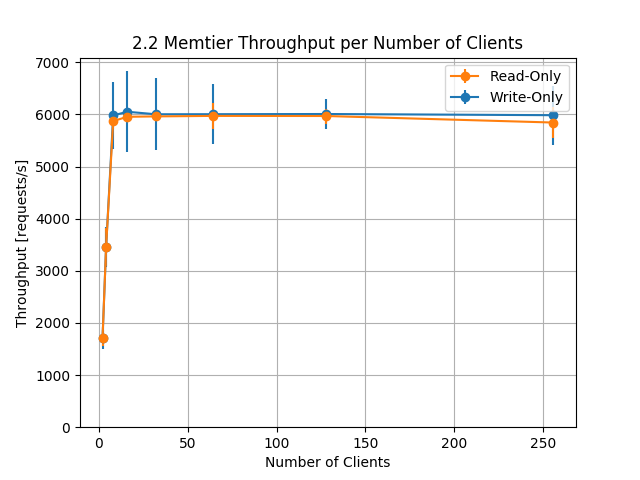
\includegraphics[width=0.5\linewidth]{figures/2_2_Memtier_Throughput_per_Number_of_Clients.png}
		\label{Figure:2_2:a}}\hfill
	\subfloat[Response time]{
		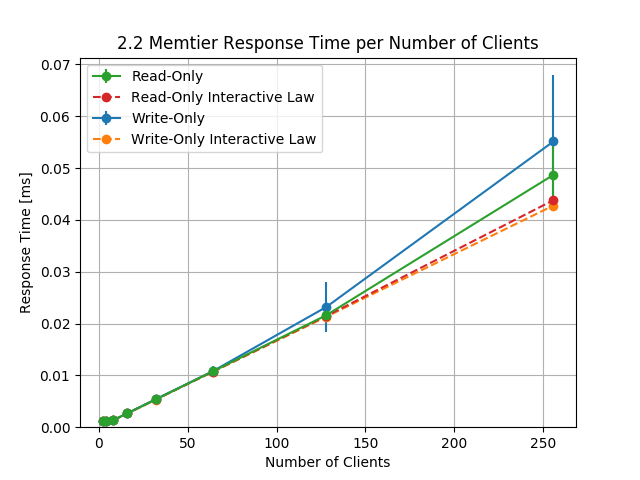
\includegraphics[width=0.5\linewidth]{figures/2_2_Memtier_Response_Time_per_Number_of_Clients.png}
		\label{Figure:2_2:b}}\\
	
	\subfloat[Network Read-Only]{
		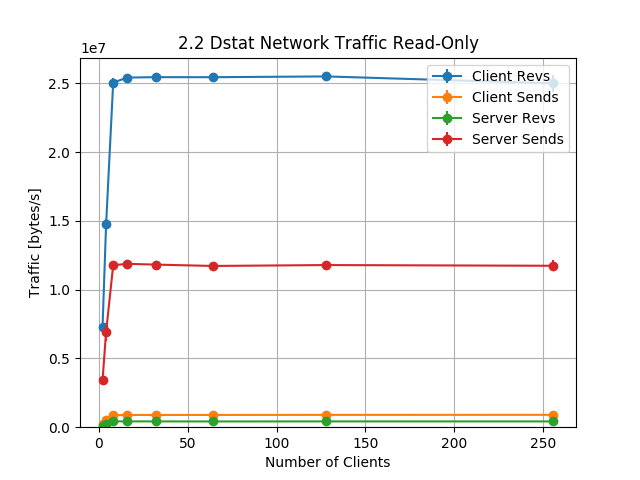
\includegraphics[width=0.5\linewidth]{figures/2_2_Dstat_Network_Traffic_Read-Only.png}
		\label{Figure:2_2_dstat:a}}\hfill
	\subfloat[Network Write-Only]{
		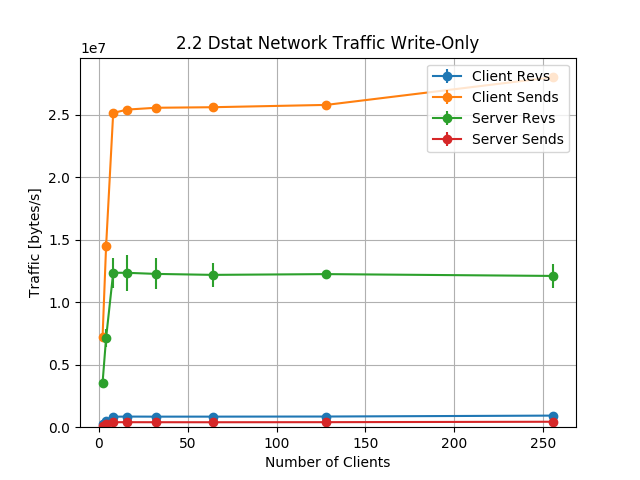
\includegraphics[width=0.5\linewidth]{figures/2_2_Dstat_Network_Traffic_Write-Only.png}
		\label{Figure:2_2_dstat:b}}\\
	\caption{\textit{Plots for experiment 2.2.} Average throughput and latency values for both a read-only and a write-only load. Also average of the network inbound and outbound traffic for clients and servers.}
	\label{Figure:2_2} 	
\end{figure}

\subsubsection{Explanation}

\mytitlesubsub[Read-Only Workload]{The throughput (see Figure \ref{Figure:2_2:a}) climbs very steeply until eight clients where it reaches saturation and from then on stays constant at around 6000 requests/sec. We can also see some oversaturation happening at 256 clients. But because the standard deviation there is substantial, this is not guaranteed to be accurate. The response time graph (see Figure \ref{Figure:2_2:b}) shows similar behaviour, changing its steepness at eight clients. The interactive law does not hold very well, as we have already seen in experiment 2.1. But again this can be explained by having some outliers with a high response time. We might expect the bottleneck to be at the client this time because we have double the servers and a third of the clients in comparison to experiment 2.1. But one client can still send around 83'300 requests/second, while both servers together can only send back around 5800 responses/second. We have to keep in mind that the client VMs have two cores while the server VMs only have one core. Thus the bottleneck is still at the server. The difference between our calculated 5800 requests/second and the measured 6000 requests/second comes from us taking the longest possible requests for the calculations and also from rounding. They still give us a good indicator though on where the bottleneck is. Looking at the traffic observed during the experiment (see Figure \ref{Figure:2_2_dstat:a}), we see this confirmed by the server outbound traffic curve correlating to the throughput curve. The client inbound traffic is twice the server outbound traffic, because we have two servers and only one client.}
\mytitlesubsub[Write-Only Workload]{The throughput (see Figure \ref{Figure:2_2:a}) looks very similar to the throughput for the read-only workload. It again climbs very steeply until eight clients where it reaches its saturation point. We can not see a point where the system gets oversaturated. We can see equal behaviour in the response time graph (see Figure \ref{Figure:2_2:b}), where there is a bend at eight clients. The interactive law does not hold as well as in the first experiment, but again the bigger error bars indicate outliers which lead to the high response time. From the similarity to the curve of the read-only workload, we might wrongly conclude that the bottleneck has to be the same. But this is just due to there being two cores at both the client side and the server side. The client can send around 5800 requests/second, while the server can handle sending back up to 250'000 responses/second. Thus the bottleneck is still at the client, just due to the high difference in length of the requests and responses. Looking at the traffic observed during the experiment (see Figure \ref{Figure:2_2_dstat:b}), we see this confirmed. The client outbound traffic curve correlates to the throughput and is twice as high as the server inbound traffic.}

\subsection{Summary}

	\begin{table}[H]
	\centering
		\begin{tabular}{|l|p{2.5cm}|p{2.5cm}|p{5.4cm}|}
			\hline                        					& Read-only workload 	& Write-only workload 	& Configuration gives max. throughput \\ 
			\hline One memcached server   &  3367.62 req/s   		&  15735.54 req/s 	 		&   \ku{numClients} = 768                                 \\ 
			\hline One load generating VM 	&   5972.33 req/s  		&  6051.57 req/s    		&  \ku{numClients} =  128 for write-only  \ku{numClients} = 32 for read-only                               \\ 
			\hline 
		\end{tabular}
		\caption{\textit{Maximum throughput for the two different experiments.}}
		\label{Table:2_table}
	\end{table}

We can see that the bottleneck is mostly due to bandwidth. In experiment 2.1 for a read-only workload, the server has to send back a long response and is thus the bottleneck. For a write-only workload the client has to send a long request and therefore the client should be the bottleneck in terms of bandwidth. But for that case we actually observe the bottleneck to be at the CPU of the server which can not handle more requests. Because the client VMs have double the amount of cores than the server VMs, we have a six to one client to server core ratio in experiment 2.1. This shows in the very high throughput for a write-only workload. The read-only workload on the other hand is limited by the single server and thus quite low. 

In experiment 2.2 we have the same number of cores on the client and server side. Thus both workloads achieve a similar throughput, both sides being the bottleneck for one of the workloads. Here we do not achieve a high enough throughput to make the CPU the bottleneck, the bottleneck is the bandwidth for both the read-only and write-only workload.

If we have one server in the system with a sufficient CPU we would actually need about 30 client machines sending SET-requests to it to finally make the server bandwidth the bottleneck. Similarly, if we had one client in the system, we would need about 20 server machines receiving GET-requests to make the client bandwidth the bottleneck.

\section{Baseline with Middleware (90 pts)}

In this section we did measurements on the throughput and latency of memtier requests with one or two middlewares. The numbers come from the logs that memtier provides, dstat, as well as our middleware logs.

\subsection{One Middleware}

The parameters are as in Table \ref{Table:3_1_table}. Throughput and latency are plotted in Figure \ref{Figure:3_1_middleware}. 

	\begin{table}[H]
	\centering
		\begin{tabular}{|l|c|}
			\hline Number of servers                					& 1                        \\ 
			\hline Number of client machines        			& 3                        \\ 
			\hline Instances of memtier per machine 		& 1                        \\ 
			\hline Threads per memtier instance     			& 2                        \\
			\hline Virtual clients per thread       				& 1, 2, 4, 8, 16, 32                  \\ 
			\hline Workload                         						& Write-only and Read-only \\
			\hline Number of middlewares            			& 1                        \\
			\hline Worker threads per middleware    		& 8, 16, 32, 64                  \\
			\hline Repetitions                      						& 3           \\ 
			\hline 
		\end{tabular}
		\caption{\textit{Parameters for experiment 3.1}}
		\label{Table:3_1_table}
	\end{table}


%\begin{figure}[ht!]
%	\subfloat[Throughput]{
%		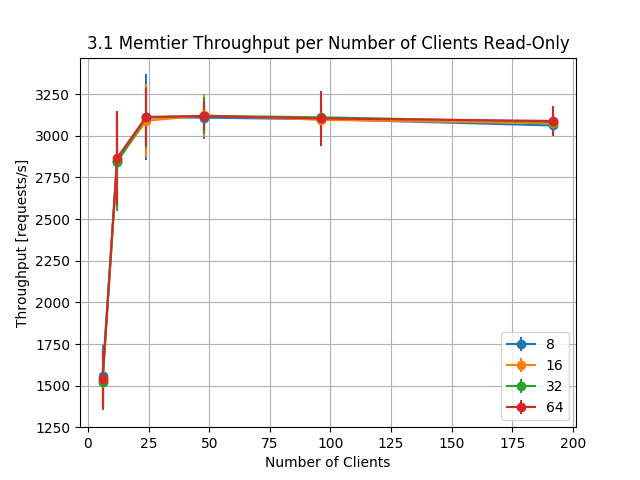
\includegraphics[width=0.5\linewidth]{3_1_Memtier_Throughput_per_Number_of_Clients.png}
%		\label{Figure:3_1_memtier:a}}\hfill
%	\subfloat[Response time]{
%		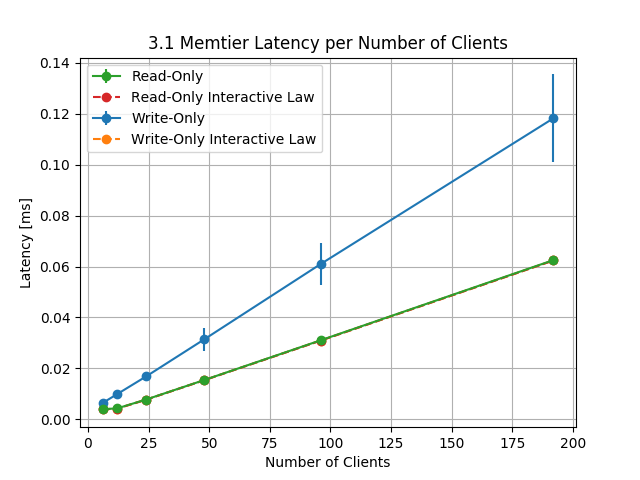
\includegraphics[width=0.5\linewidth]{3_1_Memtier_Latency_per_Number_of_Clients.png}
%		\label{Figure:3_1_memtier:b}}\\
%	\caption{dddd}
%	\label{Figure:3_1_memtier} 	
%\end{figure}

\begin{figure}[]
	\subfloat[Throughput Read-Only]{
		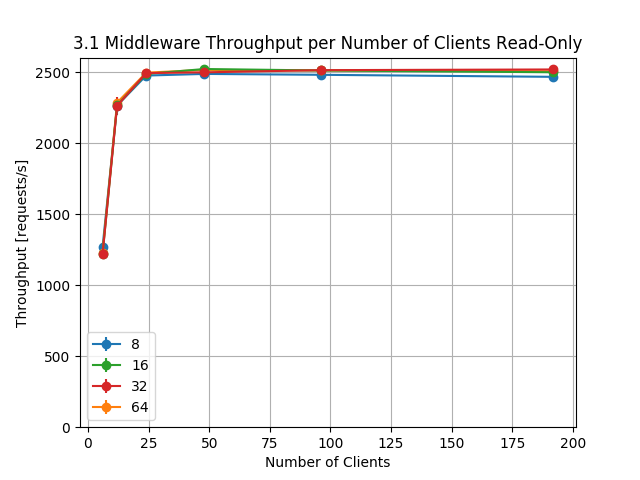
\includegraphics[width=0.5\linewidth]{figures/3_1_Middleware_Throughput_per_Number_of_Clients_Read-Only.png}
		\label{Figure:3_1_middleware:a}}\hfill
		\subfloat[Throughput Write-Only]{
		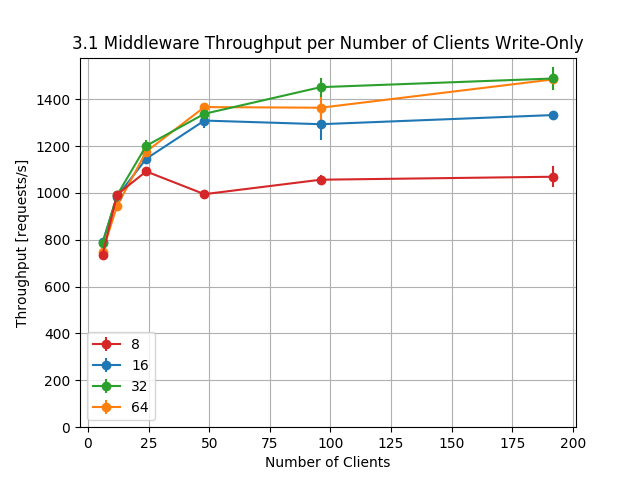
\includegraphics[width=0.5\linewidth]{figures/3_1_Middleware_Throughput_per_Number_of_Clients_Write-Only.png}
		\label{Figure:3_1_middleware:d}}\hfill
	
	
	\subfloat[Response Time Read-Only]{
		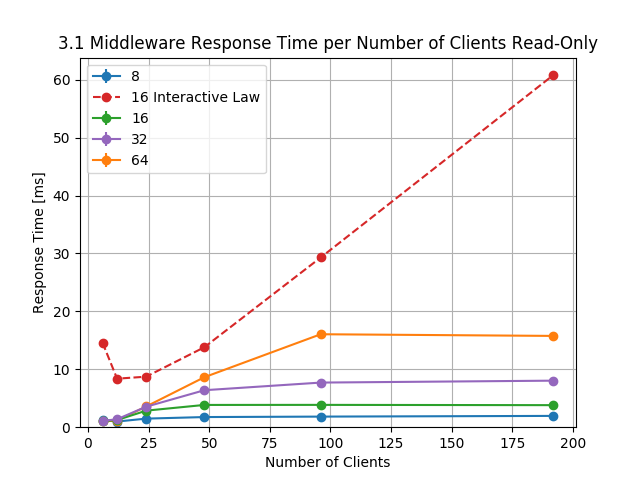
\includegraphics[width=0.5\linewidth]{figures/3_1_Middleware_Response_Time_per_Number_of_Clients_Read-Only.png}
		\label{Figure:3_1_middleware:b}}\hfill
	\subfloat[Response Time Write-Only]{
		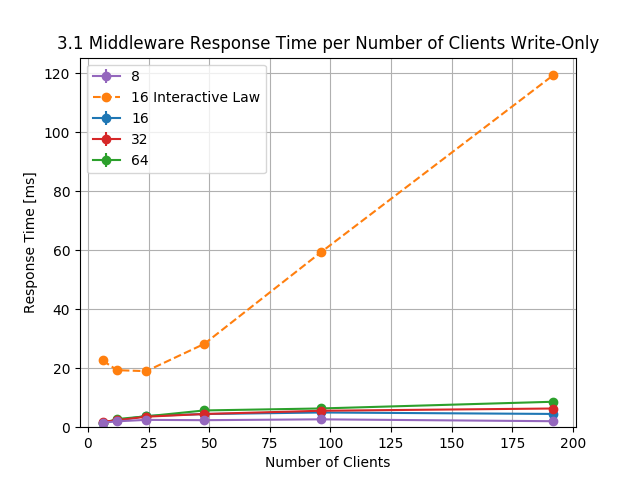
\includegraphics[width=0.5\linewidth]{figures/3_1_Middleware_Response_Time_per_Number_of_Clients_Write-Only.png}
		\label{Figure:3_1_middleware:e}}\hfill	
	
	\subfloat[Queue Length Read-Only]{
		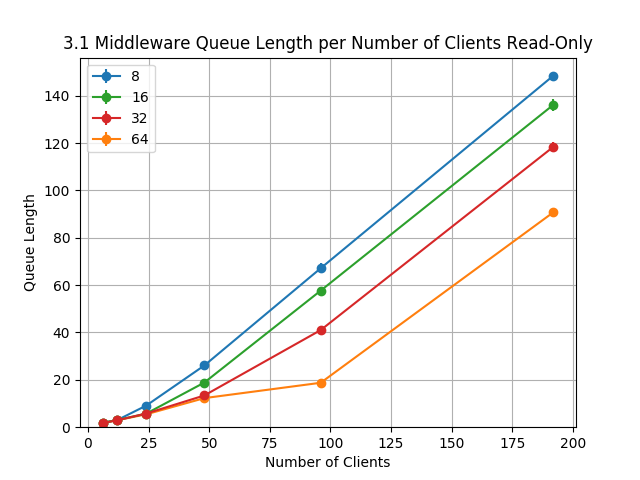
\includegraphics[width=0.5\linewidth]{figures/3_1_Middleware_Queue_Length_per_Number_of_Clients_Read-Only.png}
		\label{Figure:3_1_middleware:c}}\hfill
	\subfloat[Queue Length Write-Only]{
		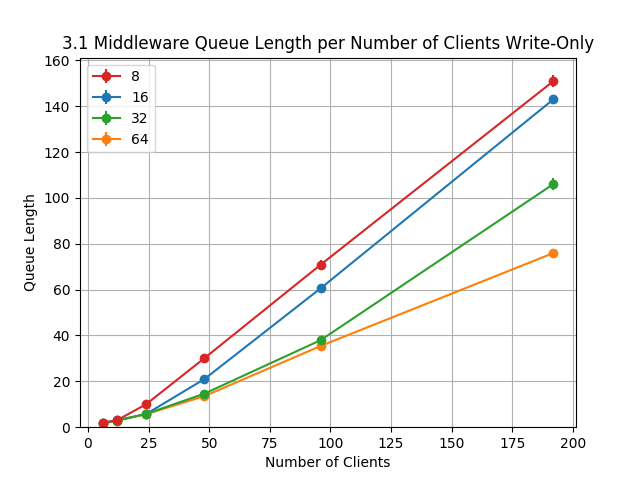
\includegraphics[width=0.5\linewidth]{figures/3_1_Middleware_Queue_Length_per_Number_of_Clients_Write-Only.png}
		\label{Figure:3_1_middleware:f}}\hfill
	\caption{\textit{Plots for experiment 3.1.} Average throughput, response time and queue length in the middleware for both a read-only and a write-only load.}
	\label{Figure:3_1_middleware} 	
\end{figure}

%\begin{figure}[ht!]
%	\subfloat[Network Read-Only]{
%		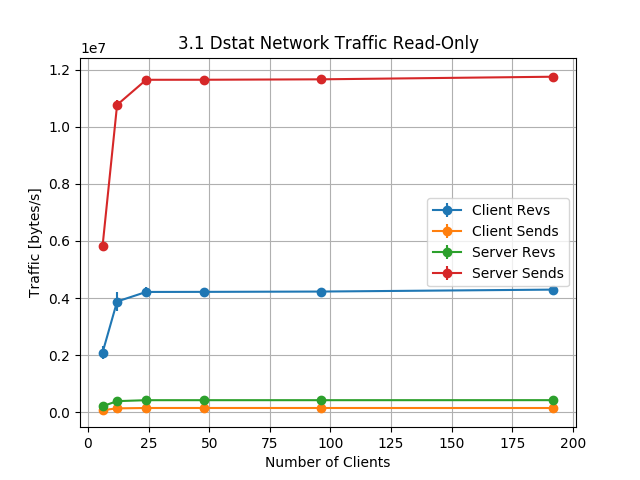
\includegraphics[width=0.5\linewidth]{3_1_Dstat_Network_Traffic_Read-Only.png}
%		\label{Figure:3_1_dstat:a}}\hfill
%	\subfloat[Network Write-Only]{
%		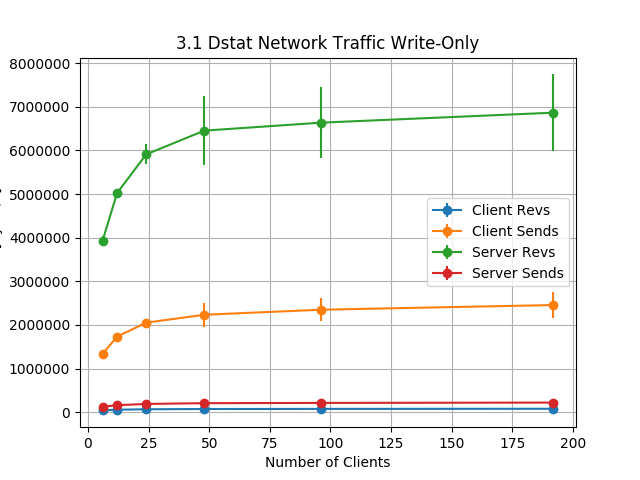
\includegraphics[width=0.5\linewidth]{3_1_Dstat_Network_Traffic_Write-Only.png}
%		\label{Figure:3_1_dstat:b}}\\
%	\caption{\textit{Network traffic measured with dstat.} Averaged the network inbound and outbound traffic for clients and servers.}
%	\label{Figure:3_1_dstat} 	
%\end{figure}

\subsubsection{Explanation}

\mytitlesubsub[Read-Only Workload]{The throughput (see Figure \ref{Figure:3_1_middleware:a}) for a read-only workload climbs very steeply until 24 clients where it reaches its saturation point. From then on it roughly stays the same for all higher number of clients. The three clients can send around 250'000 requests/second, the midddleware can send a bit less at around 166'700 requests/second, but most importantly the server can only send back about 2900 responses/second. Thus the bottleneck is actually still the server, even though we measured a throughput of only around 2500. This will become clear after looking at experiment 3.2. The response time (see Figure \ref{Figure:3_1_middleware:b}) stays at about 4 ms for 6 and 12 clients, then starts to increase. The increase depends on the number of middleware threads, getting bigger faster for a higher number of threads. The  response time for 8, 16 and 32 middleware threads reaches its maximum at 48 clients. For 64 clients it is reached at 96 clients. The reason that the response time can get longer while the throughput stays the same is that doubling the amount of requests in the system while also doubling the response time results in the same throughput. Looking at the queue length (see Figure \ref{Figure:3_1_middleware:c}) confirms this. From the point on where we reach maximum throughput, the queue length starts to grow linearly. This shows that requests start to pile up in the queue, with the server not being able to handle the load. The interactive law gives an upper bound as it should. The difference between the measured values and the predicted values can be explained with the thinking time not being zero as is assumed while calculating the law. The only point where there is another significant offset is at 6 clients. This is because there are more middleware threads than clients, leaving at least two middleware threads idle at all times. We do not take this into account when calculating the interactive law as number of middleware threads over throughput, resulting in this difference.}

\mytitlesubsub[Write-Only Workload]{The throughput (see Figure \ref{Figure:3_1_middleware:d}) for a write-only workload climbs steeply until 24 clients, then the curves start to stabilize in order from least middleware threads to most. For 64 middleware threads, we cannot really see a saturation point as it is still climbing from 96 to 192 clients. The response time (see Figure \ref{Figure:3_1_middleware:e}) shows similar behaviour as for the read-only workload, but is overall shorter. The queue length (see Figure \ref{Figure:3_1_middleware:f}) gets longer faster, the less middleware threads we have to handle the request that are piling up in the queue. The three clients can send around 17'400 requests/second, the middleware can send a bit less at around 11'700 requests/second and the server can handle sending back up to 125'000 responses/second. Our measured values are much lower than that, which has its cause in our implementation of the middleware which introduces a huge overhead. The reason why the middleware is only the bottleneck for the write-only workload is that it takes much longer to parse a SET request than it takes to parse a GET request, because it has to look at the content of the request to make sure that it is complete. The middleware is still faster than the server for a read-only workload. The interactive law predicts a much longer response time than was measured. We can explain this again with the thinking time. This time is even longer for SET requests than for GET requests, again because our middleware handles it differently. The small spike at 6 clients is explained the same way as for the read-only workload.} 

\subsection{Two Middlewares}

The parameters are as in Table \ref{Table:3_2_table}. Throughput and latency are plotted in Figure \ref{Figure:3_2_middleware}. 

	\begin{table}[H]
	\centering
		\begin{tabular}{|l|c|}
			\hline Number of servers                				& 1                        \\ 
			\hline Number of client machines        		& 3                        \\ 
			\hline Instances of memtier per machine 	& 2                        \\ 
			\hline Threads per memtier instance     		& 1                        \\
			\hline Virtual clients per thread       			& 1, 2, 4, 8, 16, 32, 64                 \\ 
			\hline Workload                         					& Write-only and Read-only \\
			\hline Number of middlewares            		& 2                        \\
			\hline Worker threads per middleware    	& 8, 16, 32, 64                 \\
			\hline Repetitions                      					& 3       \\ 
			\hline 
		\end{tabular}
		\caption{\textit{Parameters for experiment 3.2}}
		\label{Table:3_2_table}
	\end{table}


%\begin{figure}[ht!]
%	\subfloat[Throughput]{
%		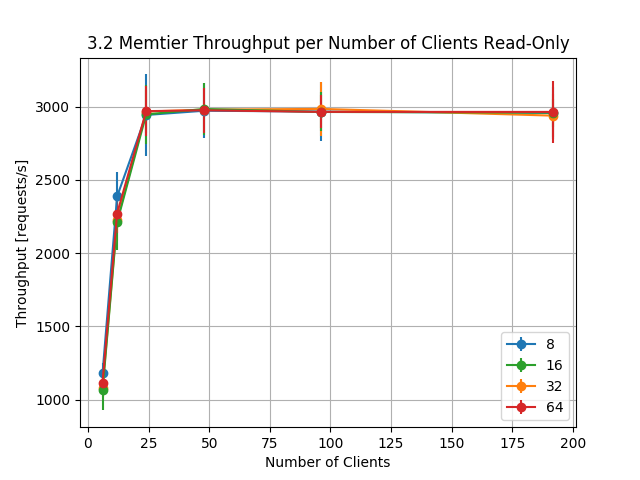
\includegraphics[width=0.5\linewidth]{3_2_Memtier_Throughput_per_Number_of_Clients.png}
%		\label{Figure:3_2_memtier:a}}\hfill
%	\subfloat[Response time]{
%		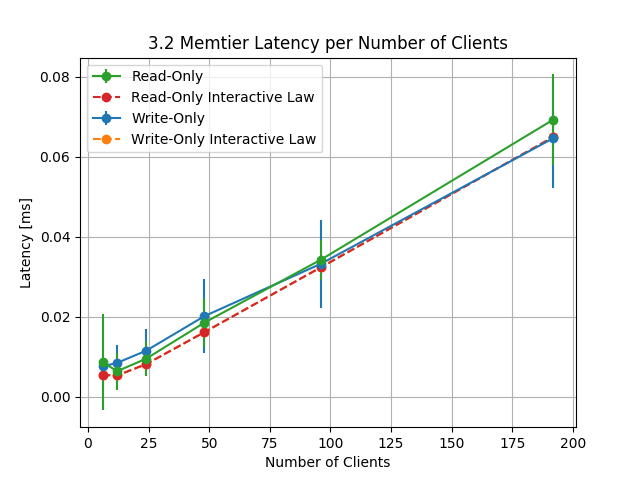
\includegraphics[width=0.5\linewidth]{3_2_Memtier_Latency_per_Number_of_Clients.png}
%		\label{Figure:3_2_memtier:b}}\\
%	\caption{dddd}
%	\label{Figure:3_2_memtier} 	
%\end{figure}

\begin{figure}[]
	\subfloat[Throughput Read-Only]{
		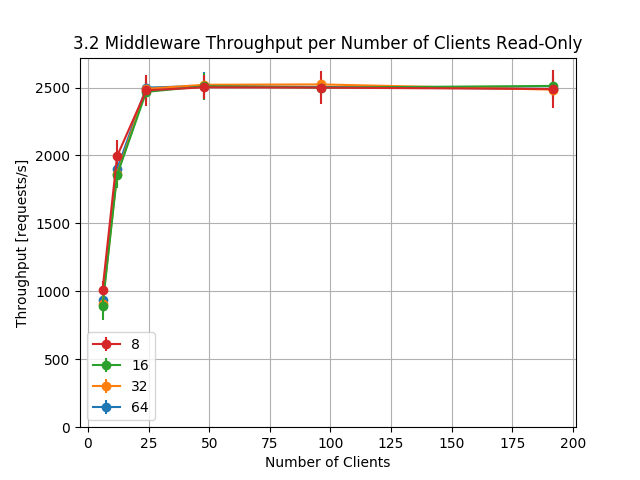
\includegraphics[width=0.5\linewidth]{figures/3_2_Middleware_Throughput_per_Number_of_Clients_Read-Only.png}
		\label{Figure:3_2_middleware:a}}\hfill
	\subfloat[Throughput Write-Only]{
		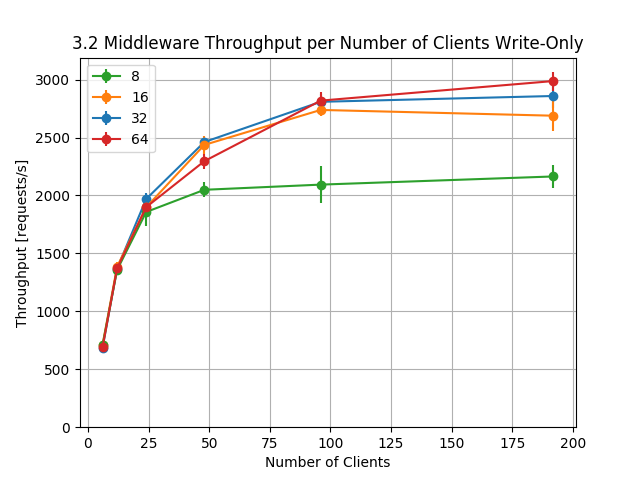
\includegraphics[width=0.5\linewidth]{figures/3_2_Middleware_Throughput_per_Number_of_Clients_Write-Only.png}
		\label{Figure:3_2_middleware:d}}\hfill
	
	\subfloat[Response Time Read-Only]{
		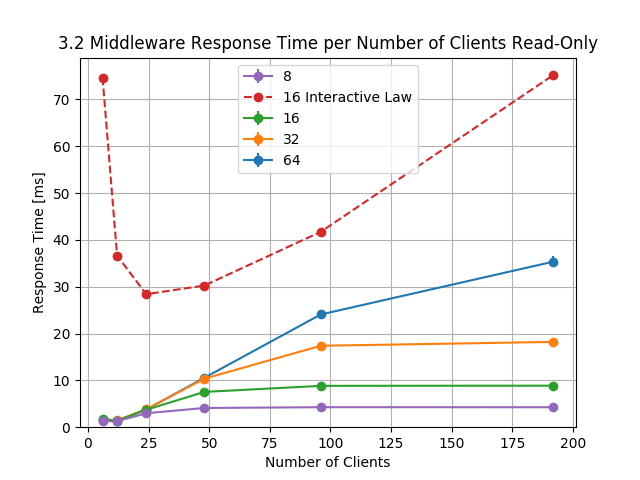
\includegraphics[width=0.5\linewidth]{figures/3_2_Middleware_Response_Time_per_Number_of_Clients_Read-Only.png}
		\label{Figure:3_2_middleware:b}}\hfill
	\subfloat[Response Time Write-Only]{
		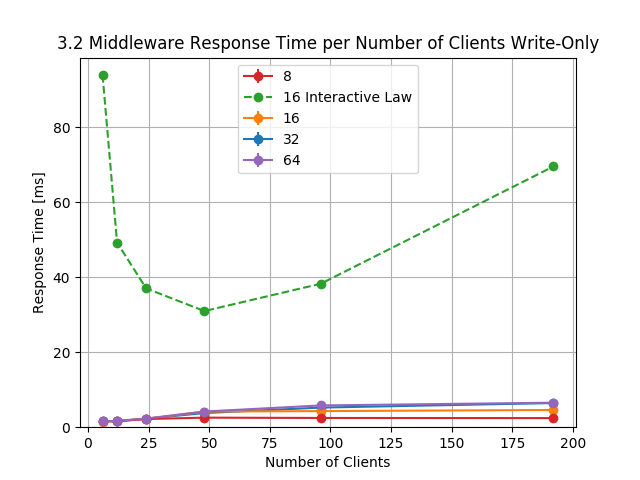
\includegraphics[width=0.5\linewidth]{figures/3_2_Middleware_Response_Time_per_Number_of_Clients_Write-Only.png}
		\label{Figure:3_2_middleware:e}}\hfill
	
	\subfloat[Queue Length Read-Only]{
		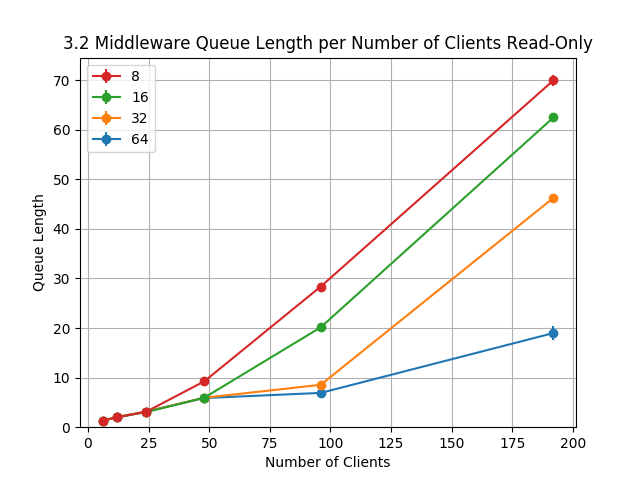
\includegraphics[width=0.5\linewidth]{figures/3_2_Middleware_Queue_Length_per_Number_of_Clients_Read-Only.png}
		\label{Figure:3_2_middleware:c}}\hfill		
	\subfloat[Queue Wait Write-Only]{
		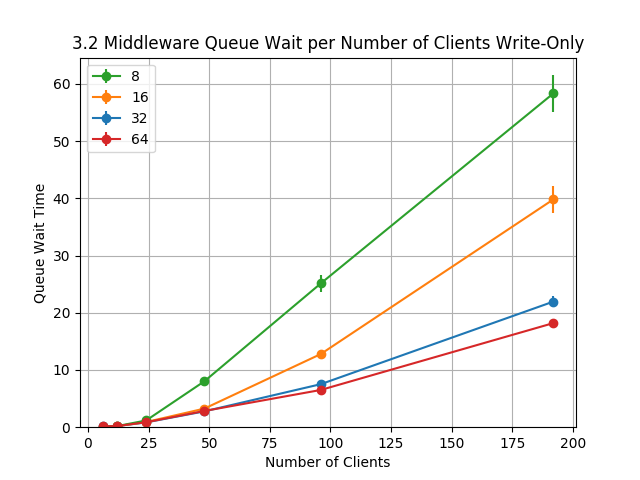
\includegraphics[width=0.5\linewidth]{figures/3_2_Middleware_Queue_Wait_per_Number_of_Clients_Write-Only.png}
		\label{Figure:3_2_middleware:f}}\hfill
	\caption{\textit{Plots for experiment 3.2.} Average throughput, response time and queue length or wait time respectively in the middleware for both a read-only and a write-only load.}
	\label{Figure:3_2_middleware} 	
\end{figure}

%\begin{figure}[ht!]
%	\subfloat[Network Read-Only]{
%		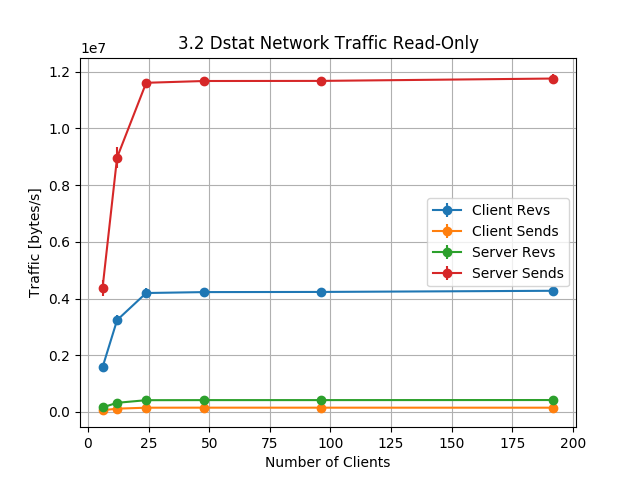
\includegraphics[width=0.5\linewidth]{3_2_Dstat_Network_Traffic_Read-Only.png}
%		\label{Figure:3_2_dstat:a}}\hfill
%	\subfloat[Network Write-Only]{
%		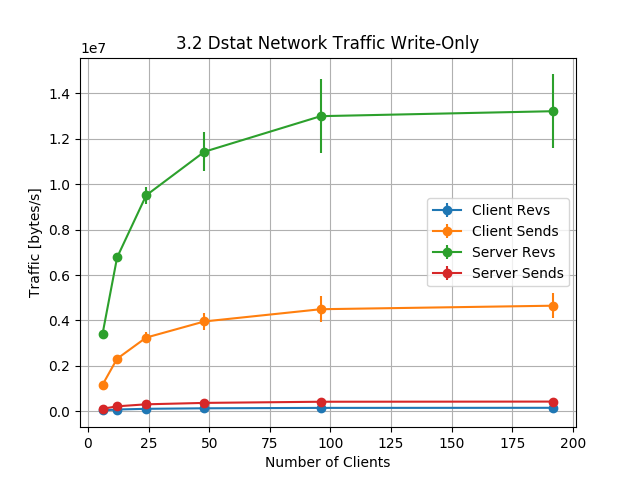
\includegraphics[width=0.5\linewidth]{3_2_Dstat_Network_Traffic_Write-Only.png}
%		\label{Figure:3_2_dstat:b}}\\
%	\caption{\textit{Network traffic measured with dstat.} Averaged the network inbound and outbound traffic for clients and servers.}
%	\label{Figure:3_2_dstat} 	
%\end{figure}


\subsubsection{Explanation}

\mytitlesubsub[Read-Only Workload]{The throughput (see Figure \ref{Figure:3_2_middleware:a}) for a read-only workload looks similar as the throughput in experiment 3.1. It also climbs steeply until we reach 24 clients and from then on roughly stays the same. It again reaches the same maximal throughput at around 2500 requests/second, which confirms again that the server is the bottleneck for read-only workloads. If the middleware was the bottleneck, we should have achieved double the throughput from experiment 3.1. The response time (see Figure \ref{Figure:3_2_middleware:b}) stays at about 2 ms for 6 and 12 clients and then begins to increase more or less steeply depending on the number of middleware threads. The maxima are reached only with twice as many clients than what we had in experiment 3.1. For 64 middleware threads we thus do not even see a inflection point yet. Correspondingly, the queue lengths (see Figure \ref{Figure:3_2_middleware:c}) also start to increase linearly only at double the clients. For example, looking at 32 middleware threads, the response time stabilizes at 96 clients and the queue length starts to linearly grow at the same point. In experiment 3.1 these two points were at 48 clients. This is all due to having only half the requests in one middleware in comparison to experiment 3.1. The interactive law is similarly inaccurate as in experiment 3.1 and this difference has the same explanation as there. The spike at 6 clients is also explained the same way.}

\mytitlesubsub[Write-Only Workload]{ The throughput (see Figure \ref{Figure:3_2_middleware:d}) for the write-only workload looks very similar to the one in experiment 3.1, also reaching a maximal throughput of around 1500 requests/second. The clients together can send around 17'400 requests/second, the middlewares together can send around 23'300 requests/second and the server can send back up to 125'000 responses/second. But again, as in experiment 3.1, the bottleneck is not because of the bandwidth, but because of the implementation of the middleware, as we have already explained in experiment 3.1. The throughput being doubled compared to experiment 3.1 supports this as well as we have doubled the number of middlewares. The queue wait time (see Figure \ref{Figure:3_2_middleware:f}) shows equivalent behaviour to the queue length in experiment 3.1, getting longer faster, the less middleware threads we have available to handle the request that are piling up in the queue. Again the interactive law is similar to experiment 3.1 and has the same explanation for why it is that way.} 

\subsection{Summary}

For the following tables, we chose the maximum throughput for the middleware and then filled in the other cells with the values that were achieved for this configuration.

	\begin{table}[H]
	\centering
		\begin{tabular}{|l|p{2cm}|p{2cm}|p{2cm}|p{2cm}|}
			\hline                                						& Throughput 	& Response time 	& Average time in queue 	& Miss rate \\ 
			\hline Reads: Measured on middleware  &  2524.40 		& 3.84					& 9.64                      			& 0          \\ 
			\hline Reads: Measured on clients     		&  3122.66        	& 15.40          		& n/a                   				&  0.06         \\ 
			\hline Writes: Measured on middleware &  1488.24        	& 8.04             		& 60.89                      		& n/a       \\ 
			\hline Writes: Measured on clients    		&  1840.66        	& 105.35             	& n/a                   				& n/a       \\ 
			\hline 
		\end{tabular}
		\caption{\textit{Maximum throughput for one middleware.} For the read-only workload, the maximum throughput was reached at 16 middleware threads and 48 clients. For a write-only workload, it was reached at 32 middleware threads and 192 clients.}
		\label{Table:3_table_1}
	\end{table}


	\begin{table}[H]
	\centering
		\begin{tabular}{|l|p{2cm}|p{2cm}|p{2cm}|p{2cm}|}
			\hline                                						& Throughput 	& Response time 	& Average time in queue 	& Miss rate \\ 
			\hline Reads: Measured on middleware  & 2523.24         &  17.39    			& 6.83                      			& 0          \\ 
			\hline Reads: Measured on clients     		& 2985.15         	&   0.03            		& n/a                   				& 0.01          \\ 
			\hline Writes: Measured on middleware & 2987.93         	&  6.53             		&  18.19                     			& n/a       \\ 
			\hline Writes: Measured on clients    		& 3628.86        	&	0.06		             	& n/a                   				& n/a       \\ 
			\hline 
		\end{tabular}
		\caption{\textit{Maximum throughput for two middlewares.} For the read-only workload, the maximum throughput was reached at 32 middleware threads and 96 clients. For a write-only workload, it was reached at 64 middleware threads and 192 clients.}
		\label{Table:3_table_2}
	\end{table}

We saw that the bottleneck for the read-only workload stays at the server for both experiments. There are two reasons for this. Our middleware is fast enough for GET-requests so that we still reach the limit of 2900 responses/second at the server. This matches with the maximum throughput we got in experiment 2.1 where also the server was the bottleneck. Using two middlewares thus does not give us any advantage for a read-only workload. The client still gets the same amount of throughput, the requests are just distributed between two middlewares. 

For a write-only workload on the other hand, the client gets double the throughput when using two middlewares, around 3600 SET-requests/second compared to around 1800 SET-requests/second with one middleware. This is because the bottleneck is actually at the middleware, thus the more middlewares we have, the more throughput we get. To shift the bottleneck away from the middlewares, we would first need to be as fast as the clients which can send around 17'400 requests per second. To do this we would need around 11 middlewares. To fully use the server, we would need round 83 middlewares sending SET-requests at full blast.

The average time in the queue reflects these observations, being longer when the middleware is the bottleneck. The cache miss rates are so low that they are negligible.

\section{Throughput for Writes (90 pts)}

In this section we did measurements on the throughput and latency of memtier SET-requests with one middleware. The numbers come from the logs that memtier provides, dstat, as well as our middleware logs.

\subsection{Full System}

The parameters are as in Table \ref{Table:4_1_table}. Throughput and latency are plotted in Figure \ref{Figure:4_1_middleware}. 

	\begin{table}[H]
	\centering
		\begin{tabular}{|l|c|}
			\hline Number of servers                					& 3          \\ 
			\hline Number of client machines        			& 3          \\ 
			\hline Instances of memtier per machine 		& 2          \\ 
			\hline Threads per memtier instance    			& 1          \\
			\hline Virtual clients per thread       				& 1, 2, 4, 8, 16, 32, 64    \\ 
			\hline Workload                         						& Write-only \\
			\hline Number of middlewares            			& 2          \\
			\hline Worker threads per middleware    		& 8, 16, 32, 64    \\
			\hline Repetitions                      						& 3  \\ 
			\hline 
		\end{tabular}
		\caption{\textit{Parameters for experiment 4.1}}
		\label{Table:4_1_table}
	\end{table}


%\begin{figure}[ht!]
%	\subfloat[Throughput]{
%		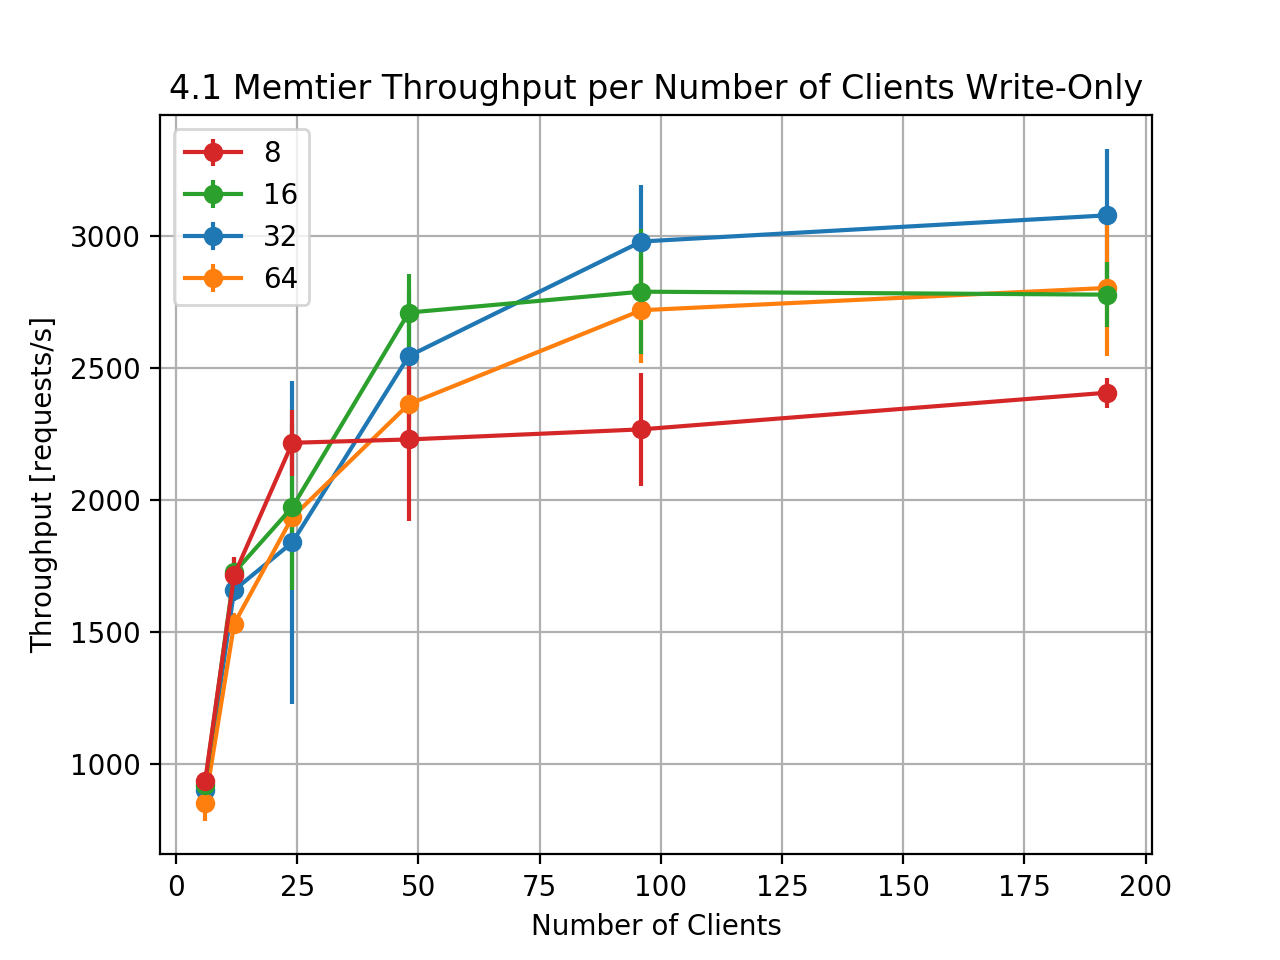
\includegraphics[width=0.5\linewidth]{4_1_Memtier_Throughput_per_Number_of_Clients.png}
%		\label{Figure:4_2_memtier:a}}\hfill
%	\subfloat[Response time]{
%		\includegraphics[width=0.5\linewidth]{4_1_Memtier_Latency_per_Number_of_Clients.png}
%		\label{Figure:4_2_memtier:b}}\\
%	\caption{dddd}
%	\label{Figure:4_2_memtier} 	
%\end{figure}

\begin{figure}[t!]
	\subfloat[Throughput Write-Only]{
		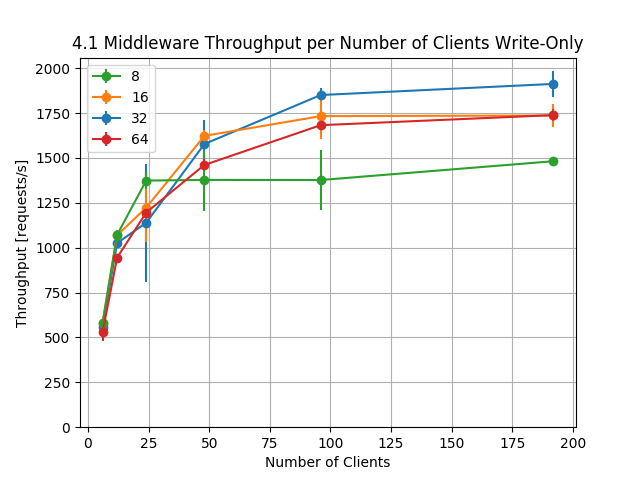
\includegraphics[width=0.5\linewidth]{figures/4_1_Middleware_Throughput_per_Number_of_Clients_Write-Only.png}
		\label{Figure:4_1_middleware:a}}\hfill
	\subfloat[Response Time Write-Only]{
		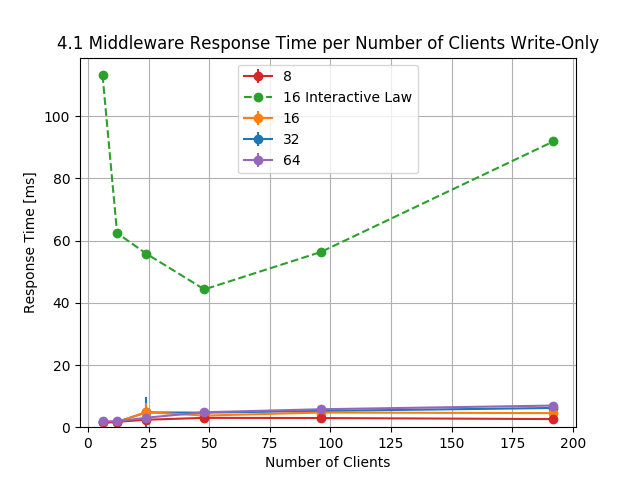
\includegraphics[width=0.5\linewidth]{figures/4_1_Middleware_Response_Time_per_Number_of_Clients_Write-Only.png}
		\label{Figure:4_1_middleware:b}}\hfill	
		
	\subfloat[Queue Wait Write-Only]{
		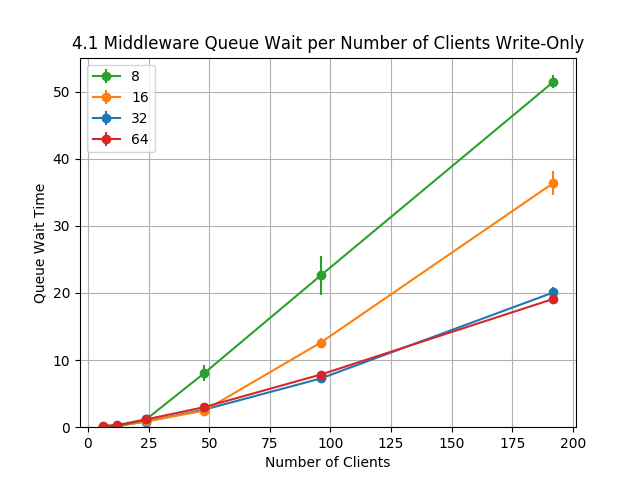
\includegraphics[width=0.5\linewidth]{figures/4_1_Middleware_Queue_Wait_per_Number_of_Clients_Write-Only.png}
		\label{Figure:4_1_middleware:c}}\hfill
	\subfloat[CPU Wait Clients]{
		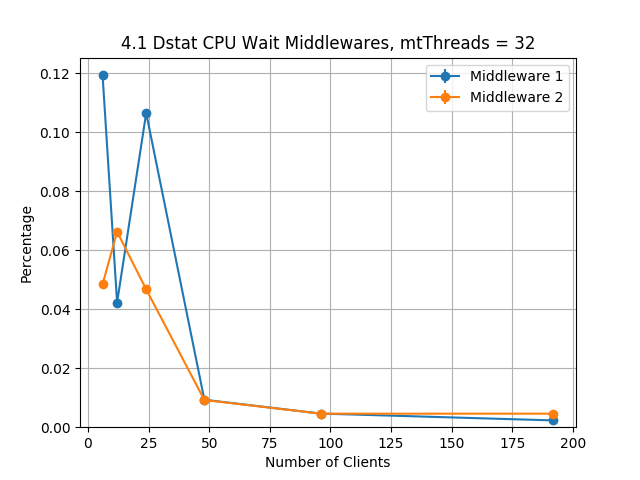
\includegraphics[width=0.5\linewidth]{figures/4_1_Dstat_CPU_Wait_Middlewares,_mtThreads_=_32.png}
		\label{Figure:4_1_dstat:a}}\hfill

	\caption{\textit{Plots for experiment 4.} Average throughput, response time and queue wait time in the middleware for both a read-only and a write-only load. Also CPU wait and software interrupt percentages in the third repetition for \ku{mtThreads=64} and \ku{numClients=6}.}
	\label{Figure:4_1_middleware} 	
\end{figure}

\subsubsection{Explanation}
The throughput (see Figure \ref{Figure:4_1_middleware:a}) grows steeply for any number of middleware threads until 24 clients. There the middleware with eight threads starts to be saturated. The middlewares with 16 and 32 threads get saturated at 96 clients and for the middleware with 64 threads we cannot make out a clear saturation point yet. The maximal throughput is less than what we achieved in experiment 3.2. Looking at the response times (see Figure \ref{Figure:4_1_middleware:b}), we note that they do not get longer in comparison to experiment 3.2. This shows that the overhead has to be in the middleware. Looking at the queue wait time (see Figure \ref{Figure:4_1_middleware:c}) can pinpoint the location of the overhead further, as they are not longer than they were in experiment 3.2, which means that the overhead has to happen after taking the request out of the queue. The reason for the overhead is that for a write-only workload we have to send the SET-request to all available servers and then aggregate the responses. Having three times as many servers as in experiment 3.2 generates an overhead. This additional overhead added to our already existing overhead for SET-requests in the middleware is also the explanation why the interacitve law  matches even worse than in experiment 3.2. The interactive law looks similar as in experiments 3.1 and 3.2 and has the same explanation why there is a big gap in between the law and the measured data.
\mytitlesubsub[Anomaly at 24 clients and 32 middleware threads] {There is a spike in the response time at this point, and when looking at the throughput we can also see that it is lower than it should be. After looking through the logs, we can pinpoint it to the first repetition in one of the middlewares. For 32 middleware threads we plot the wait time of the CPUs in the middlewares in Figure \ref{Figure:4_1_dstat:a} and can see that one of the middlewares has a spike at 24 clients. This means that one of the middlewares is waiting for an IO operation to complete. This is most likely due to having problems sending a request to the servers.}

\subsection{Summary}

For the following table, we chose the maximum throughput for the middleware and then filled in the other cells with the values that were achieved for this configuration.

\begin{table}[H]
	\centering
	\begin{tabular}{|l|p{1.5cm}|p{1.5cm}|p{1.5cm}|p{1.5cm}|}
		\hline                                            										& WT=8 		& WT=16 		& WT=32 		& WT=64 \\ 
		\hline Throughput (Middleware)                    					& 1482.09	 	& 1736.83	     & 1912.82    	& 1739.05      \\ 
		\hline Throughput (Derived from MW response time) 	& 3060.72    & 3535.13  	& 5177.62   	& 9201.62     \\ 
		\hline Throughput (Client)                        						& 2405.39  	& 2776.89   	& 3077.39   	& 2802.34       \\ 
		\hline Average time in queue                     						& 51.45     	& 36.38     	& 20.08      	& 19.12      \\ 
		\hline Average length of queue                    					& 55.86     	& 47.80      	& 30.78      	& 29.06      \\ 
		\hline Average time waiting for memcached         			& 2.61    		& 4.53      		& 6.18      		& 6.96      \\ 
		\hline 
	\end{tabular}
	\caption{\textit{Maximum throughput for the full system.} For all middleware threads, the maximum throughput was achieved with 192 clients. }
	\label{Table:4_table}
\end{table}

The throughput for 16 and 64 middleware threads is almost the same, but the average time in the queue and the length of the queue are almost halved. This makes sense as there are more worker threads taking requests from the queue and processing them at the same time. The bottleneck in this experiment is the middleware, as was expected after it was also the bottleneck in experiment 3.2 and adding two more servers only reduces the throughput because of the overhead that is created by sending the requests to all three servers.

\section{Gets and Multi-gets (90 pts)}

In this section we did measurements on the throughput and latency of memtier GET-requests with two middlewares. We did experiments for both the sharded and non-sharded behaviour. The numbers come from the logs that memtier provides, dstat, as well as our middleware logs. All plots in this section only take into account the GET-requests, SET-requests are not included in the response times.

\subsection{Sharded Case}

The parameters are as in Table \ref{Table:5_1_table}. The latency is plotted in Figure \ref{Figure:5_1}.

\begin{table}[H]
	\centering
		\begin{tabular}{|l|c|}
			\hline Number of servers                						& 3                       \\ 
			\hline Number of client machines        				& 3                       \\ 
			\hline Instances of memtier per machine 			& 2                       \\ 
			\hline Threads per memtier instance     				& 1                       \\
			\hline Virtual clients per thread       					& 2     		            \\ 
			\hline Workload                         							& ratio=1:$<$Multi-Get size$>$           \\
			\hline Multi-Get behavior               						& Sharded                 \\
			\hline Multi-Get size                  							& 1, 3, 6, 9                \\
			\hline Number of middlewares           					& 2                       \\
			\hline Worker threads per middleware    			& 32 \\
			\hline Repetitions                     							& 3      \\ 
			\hline 
		\end{tabular}
	\caption{\textit{Parameters for experiment 5.1}}
	\label{Table:5_1_table}
\end{table}

\begin{figure}[H]
	\centering
	\subfloat[Client response time for sharded]{
		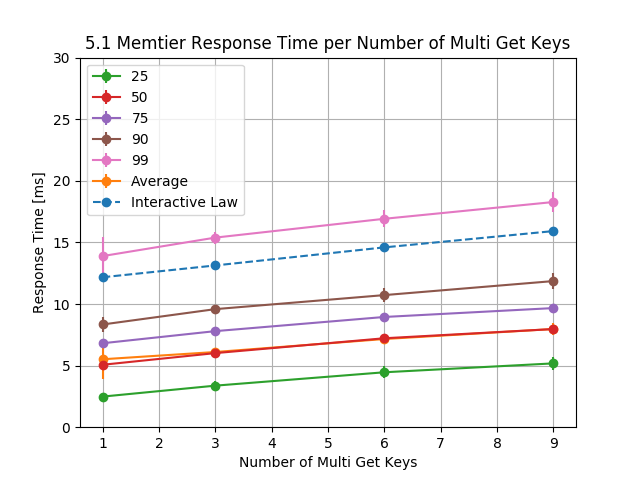
\includegraphics[width=0.45\linewidth]{figures/5_1_Memtier_Response_Time_per_Number_of_Multi_Get_Keys.png}
		\label{Figure:5_1:a}}\hfill
	\subfloat[Middleware response time for sharded]{
		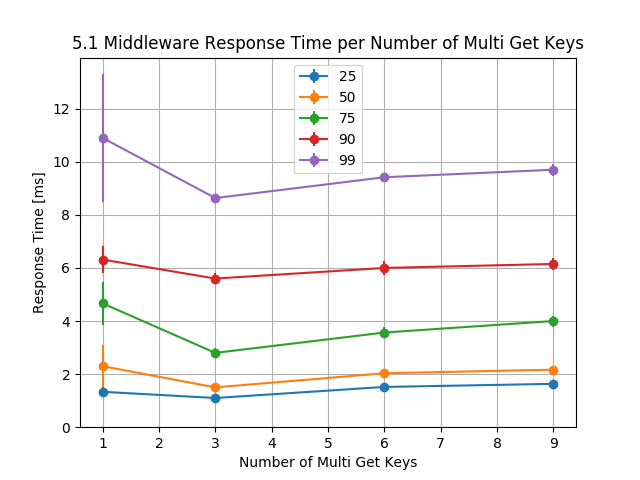
\includegraphics[width=0.45\linewidth]{figures/5_1_Middleware_Response_Time_per_Number_of_Multi_Get_Keys.png}
		\label{Figure:5_1:b}}
	\caption{\textit{Plots for experiment 5.1.} Average response time and the \nth{25}, \nth{50}, \nth{75}, \nth{90} and \nth{99} percentiles for the sharded case, both measured at the client and at the middleware.}
	\label{Figure:5_1} 	
\end{figure}

\subsubsection{Explanation}

\mytitlesubsub[Sharded Mode in the Middleware]{Having sharding enabled introduces a lot of overhead into the middleware. For a non-sharded GET-request, we simply choose one server by hashing on the first key, send it to that server and forwarding the response we get to the client. A sharded GET-request with multi-get size one works exactly like a normal single GET-request. Thus from now on we discuss the sharded GET-requests with multi-get size bigger than one. For a sharded GET-request, we have to first calculate the number of requests we send to each of the available servers. In this experiment every server gets the same number of requests, but this is only the case if the multi-get size is a multiple of the number of available servers. Generally we have to compute it using the formulas as described in section 1.3.2. Doing this takes quite some time already. After that we have to actually build the new GET-requests by splitting the original GET-request into pieces. After that we have to send the requests to all servers (or only a subset, if the multi-get size is smaller than the number of available servers) and then wait for a response from each one. We then have to construct a new response out of all the responses, making sure we put them in the right order. After that we can finally send the response back to the client.}

\mytitlesubsub[Explanation of the Response Time]{Seeing how much work this is it is not a surprise that the response time at the client increases with the multi-get size, as we can see in Figure \ref{Figure:5_1:a}. The average is right on the \nth{50} percentile, indicating a very balanced response time. The small error bars support this as well. Looking at the \nth{99} percentile for the response time as measured in the middleware (see Figure \ref{Figure:5_1:b}), we see that the response time is a bit smaller for multi-get size three than for a single GET-request and then starts to get slower again for multi-get sizes six and nine. The single GET-request response time has a big error bar, indicating some outliers. The other three values though behave like expected. From the difference in the steepness of the slopes in the client response time and the middleware response time we can again confirm that there is an overhead in the middleware. The interactive law predicts more than double of what we measured. This is easily explained, because we do not take into account the SET-requests that are happening, so they are essentially treated as think time. As we assume think time zero for the interactive law it cannot accurately predict the response time.}

\subsection{Non-sharded Case}

The parameters are as in Table \ref{Table:5_2_table}. Throughput and latency are plotted in Figure \ref{Figure:5_2}.

\begin{table}[H]
	\centering
		\begin{tabular}{|l|c|}
			\hline Number of servers                						& 3                       \\ 
			\hline Number of client machines        				& 3                       \\ 
			\hline Instances of memtier per machine 			& 2                       \\ 
			\hline Threads per memtier instance     				& 1                       \\
			\hline Virtual clients per thread       					& 2     		            \\ 
			\hline Workload                         							& ratio=1:$<$Multi-Get size$>$           \\
			\hline Multi-Get behavior               						& Non-Sharded                 \\
			\hline Multi-Get size                  							& 1, 3, 6, 9                \\
			\hline Number of middlewares           					& 2                       \\
			\hline Worker threads per middleware    			& 32 \\
			\hline Repetitions                     							& 3      \\ 
			\hline 
		\end{tabular}
	\caption{\textit{Parameters for experiment 5.2}}
	\label{Table:5_2_table}
\end{table}

\begin{figure}[H]
	\centering
	\subfloat[Response time]{
		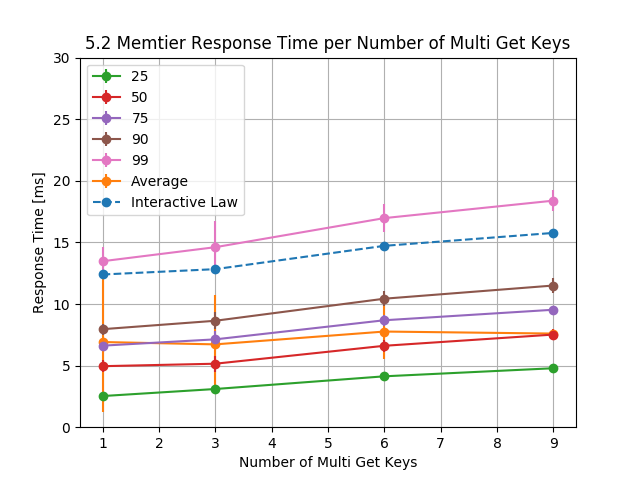
\includegraphics[width=0.3\linewidth]{figures/5_2_Memtier_Response_Time_per_Number_of_Multi_Get_Keys.png}
		\label{Figure:5_2:a}}\hfill
	\subfloat[CPU Usage on the servers]{
		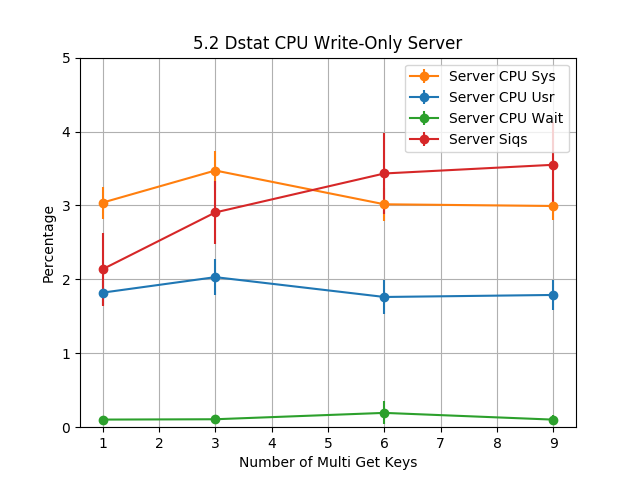
\includegraphics[width=0.3\linewidth]{figures/5_2_Dstat_CPU_Write-Only_Server.png}
		\label{Figure:5_2:b}}\hfill
	\subfloat[Network receives on the servers]{
		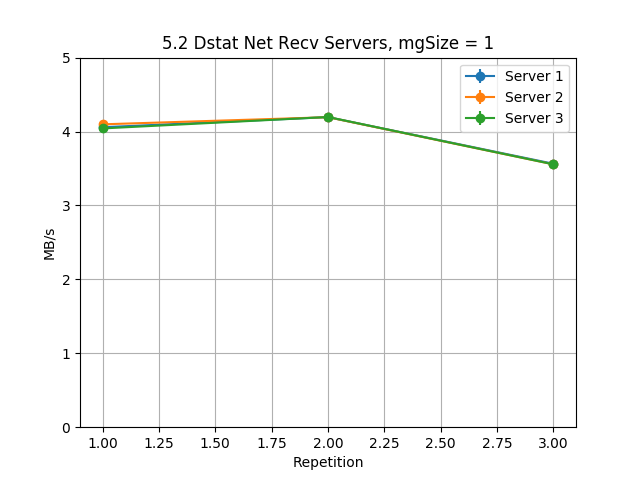
\includegraphics[width=0.3\linewidth]{figures/5_2_Dstat_Net_Recv_Servers,_mgSize_=_1.png}
		\label{Figure:5_2:c}}\hfill
	\caption{\textit{Plots for experiment 5.2.} Average response time and the \nth{25}, \nth{50}, \nth{75}, \nth{90} and \nth{99} percentiles for the non-sharded case measured at the client as well as the CPU usage on the servers. Also shown is the network income traffic at the servers for multi-get key size one.}
	\label{Figure:5_2} 	
\end{figure}

\subsubsection{Explanation}

\mytitlesubsub[Non-Sharded Mode in the Middleware]{When sharding is not enable in the middleware, a MULTI-GET-request behaves exactly the same as a single GET-request. We simply select a server to send it to via a hash function, wait for a response and forward that to the client.}

\mytitlesubsub[Explanation of Response Time]{Because we do not have much of an overhead in the middleware, we would expect the response time to grow for bigger multi-get sizes as they take more time to be responded to by the single server. Looking at the response times measured at the client (see Figure \ref{Figure:5_2:a}) we see that this is true, we can see an increase in response time for bigger multi-get sizes. We see the increase of work at the server in Figure \ref{Figure:5_2:b} where the server interrupts increase for a bigger multi-get size. Our average for multi-get size one has a very high error bar. Looking into the log files we can determine the source of this to be the third repetition where there was a period of nearly 20 seconds where all clients had a much smaller throughput through both of the middlewares. Both middlewares also logged a period of much smaller throughput at the same time. The error thus has to be either at the server or in the connection between the middleware and the server. Looking at how much the server receives for multi-get size one over the three repetitions (see Figure \ref{Figure:5_2:c}) we can clearly see that it is much smaller in the third repetition for all three servers. Thus something has to have happened in the network between the middlewares and the servers. The interactive law again predicts a higher response time than what was measured. This can be explained the same as for the sharded mode.}

\subsection{Histogram}

\begin{figure}[H]
	\centering
	\subfloat[Histogram memtier]{
		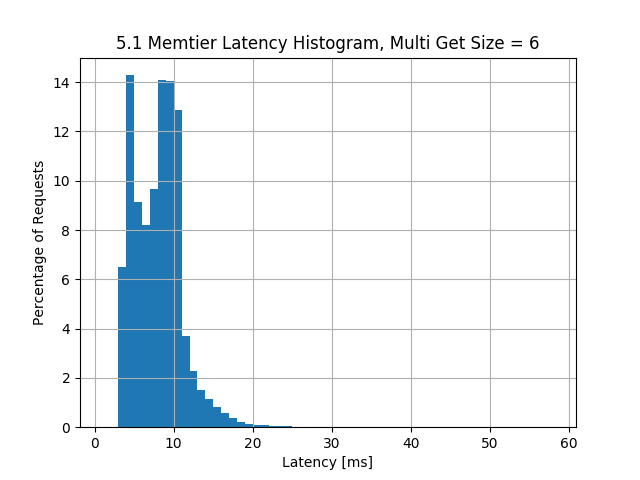
\includegraphics[width=0.45\linewidth]{figures/5_1_Memtier_Latency_Histogram,_Multi_Get_Size_=_6_png.png}
		\label{Figure:5_1_hist:a}}\hfill
	\subfloat[Histogram middleware]{
		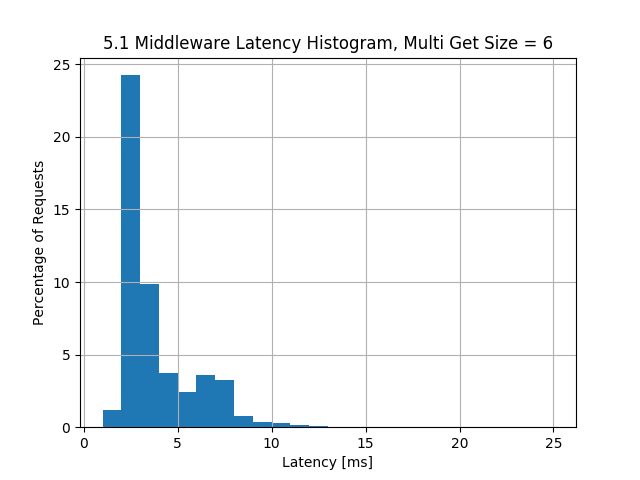
\includegraphics[width=0.45\linewidth]{figures/5_1_Middleware_Latency_Histogram,_Multi_Get_Size_=_6_png.png}
		\label{Figure:5_1_hist:b}}
	\caption{\textit{Histograms for experiment 5.1.} Histograms for multi-get size six, both measured at the client and at the middleware.}
	\label{Figure:5_1_hist} 	
\end{figure}

\begin{figure}[H]
	\centering
	\subfloat[Histogram memtier]{
		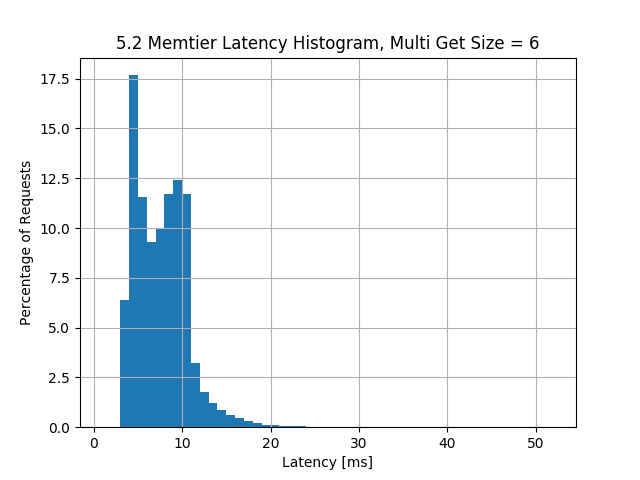
\includegraphics[width=0.45\linewidth]{figures/5_2_Memtier_Latency_Histogram,_Multi_Get_Size_=_6_png.png}
		\label{Figure:5_2_hist:a}}\hfill
	\subfloat[Histogram middleware]{
		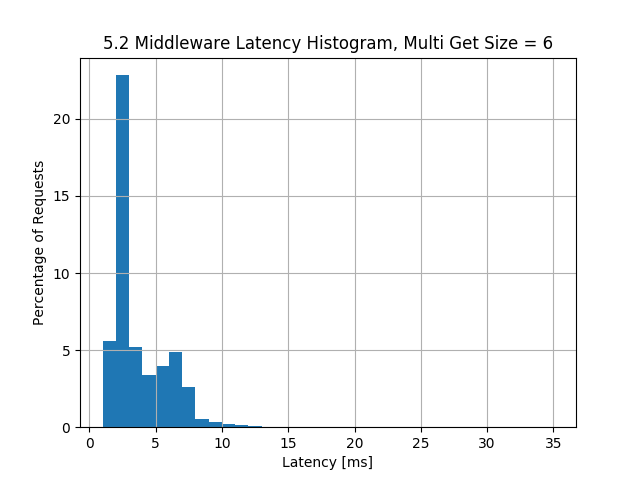
\includegraphics[width=0.45\linewidth]{figures/5_2_Middleware_Latency_Histogram,_Multi_Get_Size_=_6_png.png}
		\label{Figure:5_2_hist:b}}
	\caption{\textit{Histograms for experiment 5.2.} Histograms for multi-get size six, both measured at the client and at the middleware.}
	\label{Figure:5_2_hist} 	
\end{figure}

\mytitle[Sharded mode]{Both histograms are plotted with a bucket size of one ms. Because we have three clients connected to two middlewares, there are six different connections. All of them can have different speeds. Looking at the histogram with the values measured on the client (see Figure \ref{Figure:5_1_hist:a}) we can see two peaks, one at 5 ms and one at 10 ms. The second peak is about double the width. Thus the first peak may be from one of the clients and the second from the other two. Comparing this with the histogram constructed from middleware measurements (see Figure \ref{Figure:5_1_hist:b}), we only see one peak there. This supports our claim that the reason for the two peaks lies between the clients and the middleware.}

\mytitle[Non-Sharded mode]{Both histograms are plotted with a bucket size of one ms. We can again see two peaks in the histogram plotted from client data (see Figure \ref{Figure:5_2_hist:a}), but this time, the second one is not as high, but even wider. Our reason for this stays the same as for the sharded case and is again supported by looking at the histogram with the values from the middlewares (see Figure \ref{Figure:5_2_hist:b}).}

\subsection{Summary}

For our middleware, the sharded and non-sharded modes both result in the same response time for the client. While the sharded mode gives a higher response time from the servers to the middleware, the overhead that is produced by splitting up the MULTI-GET request cancels out this advantage. Because the simple mode of just sending the whole request to one server performs equally as good, we would not use sharding at all giving us a much simpler middleware.

\section{2K Analysis (90 pts)}

The parameters are as in Table \ref{Table:6_table}. The parameters we investigate are a the number of memcached servers, the number of middlewares and the number of middleware threads.

\begin{table}[H]
	\centering
		\begin{tabular}{|l|c|}
			\hline Number of servers                				& 1 and 3                                     \\ 
			\hline Number of client machines        		& 3                                           \\ 
			\hline Instances of memtier per machine 	& 1 (1 middleware) or 2 (2 middlewares)                                           \\ 
			\hline Threads per memtier instance     		& 2 (1 middleware) or 1 (2 middlewares)                                          \\
			\hline Virtual clients per thread       			& 32                                     \\ 
			\hline Workload                         					& Write-only and Read-only \\
			\hline Number of middlewares            		& 1 and 2                                     \\
			\hline Worker threads per middleware    	& 8 and 32                                    \\
			\hline Repetitions                      					& 3                                 \\ 
			\hline 
		\end{tabular}
	\caption{\textit{Parameters for experiment 6.}}
	\label{Table:6_table}
\end{table}

\mytitle[Choice of model]{The first decision that has to be made when doing a 2K analysis is to choose between an additive and a multiplicative model. We know that the number of middlewares and the number of middleware threads are not independent from each other. Using double the number of middlewares also doubles the number of middleware threads. The number of servers is independent from the others and thus should be modelled additively. Because we cannot mix the two models, we chose the multiplicative model, because two of the three parameters should be modelled that way.

In the following tables, MT stands for number of middleware threads, MW stands for number of middlewares and S stands for number of servers.

We are actually doing a 2kr analysis, as we are doing multiple repetitions for each experiment.}
\begin{table}[H]
\centering
\begin{tabular}{| l | r | r |}
\hline
			                              			& Throughput	& Response Time	\\ \hline
MT                       						& 0.97 \%         				& 0.37\%	\\ \hline
MW                         					& 5.56 \%         				& 10.67\%	\\ \hline
S                       							& 86.74 \%         			& 76.93\%	\\ \hline
MT $\cdot$ MW           				& 0.45 \%         				& 0.07\%\\ \hline
MT $\cdot$ S      						& 0.29 \%         				& 0.01\%\\ \hline
MW $\cdot$ S            				& 5.37 \%         				& 10.15 \%	\\ \hline
MT $\cdot$ MW $\cdot$ S 		& 0.38 \%        				& 0.01\%\\ \hline
Error                              				& 0.238 \%         			& 1.772\%\\  \hline
\end{tabular}
\caption{\textit{Read-Only 2kr Analysis Results.} Throughput and response time for a read-only workload.}
\label{Table:6_1}
\end{table}

\mytitle[Read-Only Workload]{In experiment 3 we saw that for a read-only workload, the bottleneck is at the server. Thus we expect that the number of servers has the biggest impact on the throughput and response time. We see this confirmed when looking at the table of the results (see Table \ref{Table:6_1}). The number of servers explains 86.74\% and 76.93\% respectively of the variation of the results. The middleware is not much behind the servers relating the amount of GET-requests it can send, so we would expect the number of middleware threads to also have an impact. Because the number of middlewares affects the number of middleware threads with a multiplicative factor, we would expect to see the bigger percentage at the number of middlewares. We see this again  confirmed in our results, the number of middlewares explains 5.56\% and 10.67\% respectively of the variation of the results and the combination of both those factors is also noticeable at 5.37\% and 10.15\% respectively. The other factors are all so low that they are negligible.}

\begin{table}[H]
\centering
\begin{tabular}{| l | r | r |}
\hline
			                              			& Throughput	& Response Time	\\ \hline
MT                       						& 9.48 \%			& 9.10 \% \\ \hline
MW                         					& 88.57 \%		& 87.57\%\\ \hline
S                       							& 0.76 \%			& 0.89\%\\ \hline
MT $\cdot$ MW           				& 0.05\%			& 0.05 \%\\ \hline
MT $\cdot$ S      						& 0.12 \%			& 0.22\%\\ \hline
MW $\cdot$ S            				& 1.38\%			& 0.01\%\\ \hline
MT $\cdot$ MW $\cdot$ S 		& 0.15\%			&0.12\%\\ \hline
Error                              				& 0.868\%		& 2.042 \%\\  \hline
\end{tabular}
\caption{\textit{Write-Only 2kr Analysis Results.} Throughput and response time for a write-only workload.}
\label{Table:6_2}
\end{table}

\mytitle[Write-Only Workload]{In experiments 3 and 4 we saw that for a write-only workload, the bottleneck is at the middleware. We would thus expect that the number of middleware threads to have the biggest impact. Because again doubling the number of middlewares doubles the number of middleware threads, we would expect the number of middlewares to have the highest percentage. Looking at the results in Table \ref{Table:6_2} we see this confirmed with the number of middlewares explaining 88.57\% and 87.57\% respectively of the variation of the results. We also expect that changing the number of middleware threads directly also changes the outcomes and again see this confirmed with it being at 9.48\% and 9.1\% respectively. The other factors are all so low that they are negligible.}

\section{Queuing Model (90 pts)}

\subsection{M/M/1}

\begin{figure}[H]
\centering
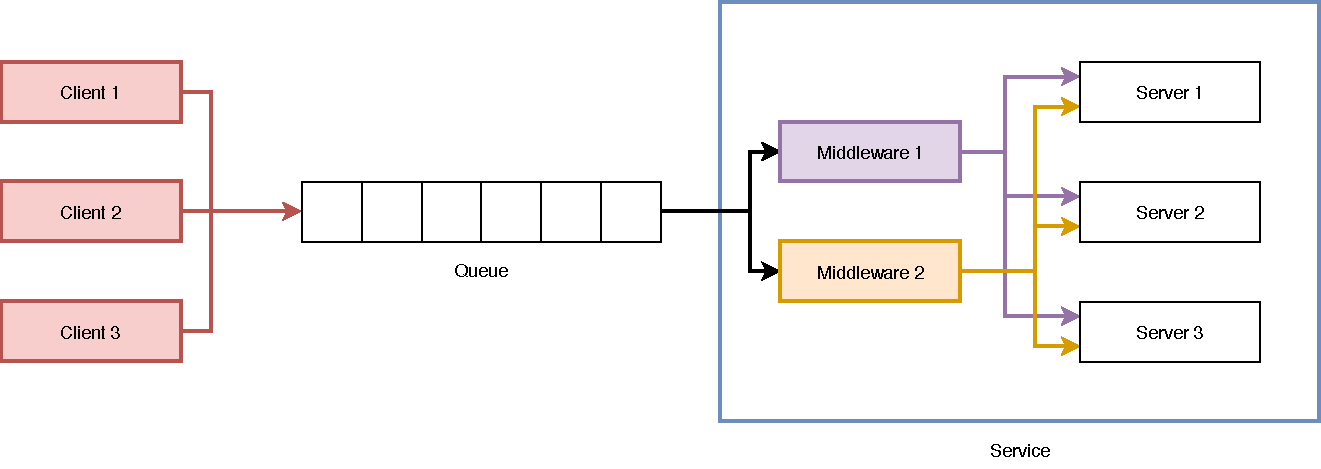
\includegraphics[width=\textwidth]{graphics/mm1.pdf}
\caption{\textit{M/M/1 Queueing Model} Illustration of how we model the setup to experiment 4 as a M/M/1 queueing model.}
\label{Figure:mm1}
\end{figure}

\mytitlesub[Choice of parameters]{We build an M/M/1 queueing model based on experiment 4, thus we have three client VMs, two middleware VMs and three server VMs. Modeling this with only one service means that the middlewares and servers are treated as one big black box before which the requests from the clients are queueing. This model is shown in Figure \ref{Figure:mm1}. We have four of these models, one for each number of middleware threads. For a M/M/1 queueing model we only need to know the arrival rate $\lambda$ and the service rate $\mu$. The state is then given by the number of jobs in the system. We choose these parameters based on what we measured in experiment 4. The mean service rate $\mu$ is the maximum observed throughput in experiment 4 over all configurations for a given number of middleware threads. The arrival rate $\lambda$ is the average throughput we observed per number of clients per number of middleware threads. Thus the service rate stays the same for one number of worker threads while the arrival rate changes. }

\mytitlesub[Computation of properties]{For an M/M/1 queue to be stable, the utilization $\rho = \frac{\lambda}{\mu}$ has to be less than 100\%. From Figure \ref{Figure:7_1:a}) we can see that this is the case for all numbers of middleware threads and thus we have a stable system. Using the utilization, we also plotted the following properties: 
\begin{equation}
\begin{split}
	\text{Mean number of jobs in the system: } & \mathbb{E}[n] = \frac{\rho}{1-\rho}\\
	\text{Mean number of jobs in the queue: } & \mathbb{E}[n_q] = \frac{\rho^2}{1-\rho}\\
	\text{Mean response time: } & \mathbb{E}[r] = \frac{1}{\mu\cdot(1-\rho)}\\
	%\text{Mean waiting time: } & \mathbb{E}[w] = \rho\frac{1}{\mu\cdot(1-\rho)}
\end{split}
\end{equation} 
}

\begin{figure}[H]
\centering
	\subfloat[Utilization of the System]{
		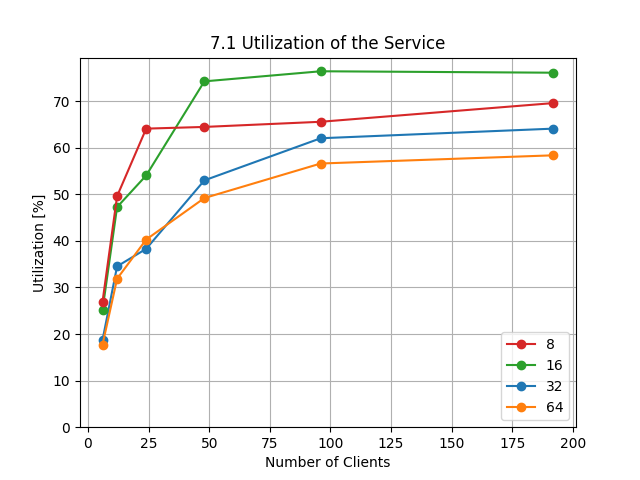
\includegraphics[width=0.45\linewidth]{figures/7_1_Utilization_of_the_Service.png}
		\label{Figure:7_1:a}}\hfill
	\subfloat[Mean Response Time]{
		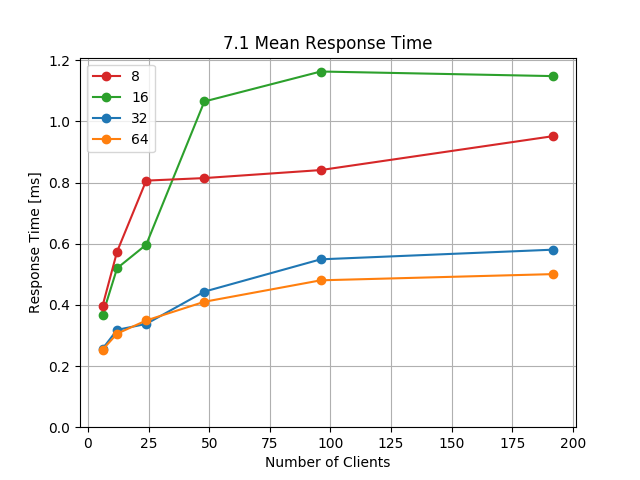
\includegraphics[width=0.45\linewidth]{figures/7_1_Mean_Response_Time.png}
		\label{Figure:7_1:d}}\hfill
		
	\subfloat[Mean Number of Jobs in the System]{
		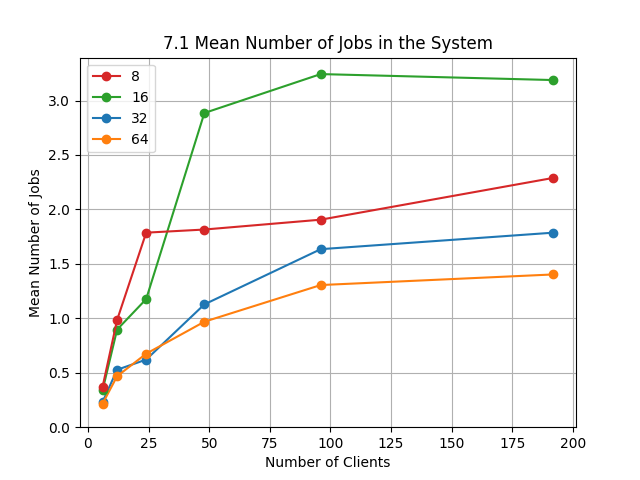
\includegraphics[width=0.45\linewidth]{figures/7_1_Mean_Number_of_Jobs_in_the_System.png}
		\label{Figure:7_1:c}}\hfill
	\subfloat[Mean Number of Jobs in the Queue]{
		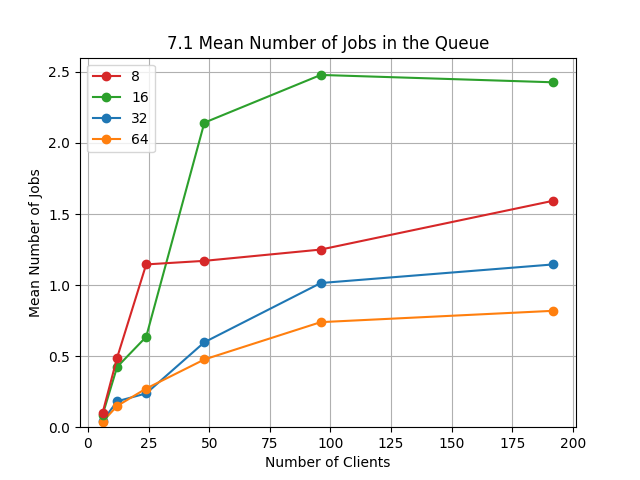
\includegraphics[width=0.45\linewidth]{figures/7_1_Mean_Number_of_Jobs_in_the_Queue.png}
		\label{Figure:7_1:b}}	
	
	%\subfloat[Mean Wait Time]{
	%	\includegraphics[width=0.45\linewidth]{7_1_Mean_Wait_Time.png}
	%	\label{Figure:7_1:e}}
	\caption{\textit{M/M/1 Queueing Model Results.} Results based on arrival rate and service rate taken from experiment 4.}
	\label{Figure:7_1} 	
\end{figure}

\mytitlesub[Comparison with measured data]{This model assumes that there is only one queue which is before the requests are handled by the \co{netThread} in one of the middlewares. Because this is not much work, the \co{netThread} can handle a lot of requests very fast, such that this queue never really builds up, as we can see in Figure \ref{Figure:7_1:d}. The queue we were talking about until now is the one inside the middleware, where requests are waiting to be picked up by a worker thread. This queue is inside the service black box and thus cannot be modelled. Because the number of jobs in the queue is so low the predicted response time (see Figure \ref{Figure:7_1:b}) is too fast. It is about half of what we measured in experiment 4. This makes sense as we actually have two queues. Another factor that plays into this is that the model does not take into account the time that it takes to get the jobs from the queue into the service and back, but instead assumes this to happen instantaneously. }

\subsection{M/M/m}

\begin{figure}[H]
\centering
\includegraphics[width=\textwidth]{graphics/mmm.pdf}
\caption{\textit{M/M/m Queueing Model} Illustration of how we model the setup of experiment 4 as a M/M/m queueing model.}
\label{Figure:mmm}
\end{figure}

\mytitlesub[Choice of parameters]{We build an M/M/m queueing model based on experiment 4, thus we have three client VMs, two middleware VMs and three server VMs. We model each of the worker threads in the middlewares as a separate service, thus we have four different values for $m$: 16, 32, 64, 128. This model is shown in Figure \ref{Figure:mmm}. For this model, we again only need the arrival rate $\lambda$ and the service rate $\mu$. We calculate $\lambda$ the same way as in the M/M/1 model, but we divide the $\mu$ used for the M/M/1 model by the number of middleware threads in the whole sytem (i.e. $m$).}

\mytitlesub[Computation of properties]{The utilization $\rho = \frac{\lambda}{m\cdot\mu}$ is shown in Figure \ref{Figure:7_2:a}. Again, because all values are below 100\% our system is in fact stable. We compute the probability of there being no jobs in the system $p_0 = \left(1+\frac{(m\rho)^m}{m!(1-\rho)}+\sum_{n=1}^{m-1}\frac{(m\rho)^n}{n!}\right)^{-1}$ and the probability  of queueing $\varrho = \frac{(m\cdot\rho)^m}{m!(a-\rho)}p_0$ and use them for plotting the following properties:
\begin{equation}
\begin{split}
	\text{Mean number of jobs in the system: } & \mathbb{E}[n] =m\cdot\rho+ \frac{\rho\cdot\varrho}{1-\rho}\\
	\text{Mean number of jobs in the queue: } & \mathbb{E}[n_q] =\varrho\frac{\rho}{1-\rho}\\
	\text{Mean response time: } & \mathbb{E}[r] = \frac{1}{\mu}\left(1+\frac{\varrho}{m\cdot(1-\rho)}\right)\\
	%\text{Mean waiting time: } & \mathbb{E}[w] = \frac{\varrho}{m\cdot\mu\cdot(1-\rho)}
\end{split}
\end{equation} 
}

\begin{figure}[H]
\centering
	\subfloat[Utilization of the System]{
		\includegraphics[width=0.45\linewidth]{figures/7_2_Utilization_of_the_Service.png}
		\label{Figure:7_2:a}}\hfill		
	\subfloat[Mean Response Time]{
		\includegraphics[width=0.45\linewidth]{figures/7_2_Mean_Response_Time.png}
		\label{Figure:7_2:d}}\hfill
	
	\subfloat[Mean Number of Jobs in the System]{
		\includegraphics[width=0.45\linewidth]{figures/7_2_Mean_Number_of_Jobs_in_the_System.png}
		\label{Figure:7_2:c}}\hfill	
	\subfloat[Mean Number of Jobs in the Queue]{
		\includegraphics[width=0.45\linewidth]{figures/7_2_Mean_Number_of_Jobs_in_the_Queue.png}
		\label{Figure:7_2:b}}\hfill		
	
	%\subfloat[Mean Wait Time]{
	%	\includegraphics[width=0.45\linewidth]{7_2_Mean_Wait_Time.png}
	%	\label{Figure:7_2:e}}
	\caption{\textit{M/M/m Queueing Model Results.} Results based on arrival rate and service rate taken from experiment 4.}
	\label{Figure:7_2} 	
\end{figure}

\mytitlesub[Comparison with measured data]{This model assumes that there is a single queue for both of the middlewares. Thus the mean number of jobs in the queue (see Figure \ref{Figure:7_2:d}) is too low. The mean number of jobs in the system (see Figure \ref{Figure:7_2:c}) is far more accurate than in the M/M/1 model. The actual values for this would be the number of worker threads, so double the number of middleware threads. Because of there being only one queue in the model instead of two, the number of jobs in the system is about half of what it should be. The utilization looks very similar to what we had for the M/M/1 model. The mean response times (see Figure \ref{Figure:7_2:b}) do not change at all for the number of clients. The cause for this could lie in the fact that the only places where the number of clients is taken into account are $\rho$ and $\varrho$. To compute the mean response time we divide these values by each other, essentially taking out the number of clients. }

\subsection{Network of Queues}

\mytitlesub[Definition of Network]{We model the setup from experiment 3 as a closed network of queues, because there are always the same number of requests in the system, equal to the number of clients. A request spends the same amount of time at the client no matter how many requests are at the client. At the same time, because each client can only hold one request, we never have a queue in front of the service. So we model it as a delay center with infinite servers. The same holds for the network between the clients and the middleware. The \co{NetThread} is a single thread whose service time does not depend on the number of requests that are queuing at the device. But there is a queue in front of it, so we model it as a M/M/1 queue which is a fixed-capacity service center. Because each \co{WorkerThread} can only take a new request after it has gotten a response from the server and sent that back to the client, we model the \co{WorkerThread}s combined with the network between the middleware and the server plus the server as one load-dependent service center. This service center is essentially a M/M/m queue.}

\begin{figure}[H]
\centering
\includegraphics[width=\textwidth]{graphics/queueNetwork.pdf}
\caption{\textit{Network of Queues} Illustration of how we model the setup of experiment 3.1 as a queue network.}
\label{Figure:queueNetwork}
\end{figure}

\mytitlesub[One Middleware]{We show in Figure \ref{Figure:queueNetwork} how our network looks for one middleware. We now have to define the service times for the different services. We do not know how fast a client on a client VM can send a new request after having sent the last one. We thus have to guess but make sure that it will not be the bottleneck. Thus we take a value of 0.01 ms. For the network we can calculate the average service time by dividing a ping by two. An average over pings measured during experiment 3 gives us an approximation of 1.1 ms for this service time. We also do not have a measurement for the \co{NetThread}, so we have to guess again. We again take the value 0.01 ms to make sure this is not the bottleneck. We calculate the service time for the \co{WorkerThread}s by dividing the number of clients by the maximum throughput of the middleware. So essentially we compute it via the interactive law. Finally for the servers we take the maximum throughput that we have seen per number of middleware threads, similar as how we defined $\mu$ in sections 7.1 and 7.2. With this choice there is no danger of our system becoming unstable because of a utilization factor bigger than one.}

\begin{figure}[]
\centering
\includegraphics[width=\textwidth]{graphics/queueNetwork2.pdf}
\caption{\textit{Network of Queues} Illustration of how we model the setup of experiment 3.2 as a queue network.}
\label{Figure:queueNetwork2}
\end{figure}

\mytitlesub[Two Middlewares]{We show in Figure \ref{Figure:queueNetwork2} how our network looks for two middlewares. The only difference is that we now have two \co{NetThread}s and two load-dependent service centers that include the \co{WorkerThread}s, network between middleware and server, and the server itself. How we define the service times stays the same. This introduces a bit of an error as actually the network and server are one and the same for both load-dependent service centers.}


\end{document}